\section{Ébullition et liquéfaction}

	\subsection{Qu’est-ce qu’un liquide ?}
	
		Un liquide est un fluide (c’est-à-dire un corps sans forme définie) dont les molécules sont très rapprochées, mais libres de se déplacer les unes par rapport aux autres.
	
		\thermoquotebegin{O}
La vapeur n’est ici qu’un moyen de transporter le calorique ; elle remplit le même office que dans le chauffage des bains par la vapeur, à l’exception que dans le cas où nous sommes son mouvement est rendu utile.
		\thermoquoteend{Sadi Carnot, 1824}{\textit{Réflexions sur la puissance motrice du feu et des machines propres à développer cette puissance}~\cite{carnot1824}}
		Concrètement, on obtient un liquide à partir d’un gaz en ralentissant et rapprochant ses molécules. Il n’y a pas de réaction chimique en jeu. Ainsi, de l’eau liquide et de la vapeur d’eau sont constituées de la même matière (des mêmes molécules) : elle est seulement assemblée différemment.
		
		Par rapport aux gaz, les liquides présentent deux différences importantes :
			\begin{itemize}
				\item Ils sont pratiquement \vocab[incompressibilité]{incompressibles}, c’est-à-dire que leur volume spécifique $v$ varie très peu lorsqu’on les compresse\footnote{Piège classique, le terme \emph{incompressible} ne veut pas dire que la pression est constante ou uniforme (bien au contraire). Il signifie seulement que le volume spécifique $v$ (et \textit{de facto} la masse volumique $\rho$) restent constants.} ;
				\item Ils sont sujets aux effets de la tension de surface, ce qui comble les esthètes et les mécanicien/nes des fluides (\cref{fig_oocestjoli}) mais est sans conséquence en thermodynamique.
			\end{itemize}
	
		\begin{figure}
			\begin{center}
				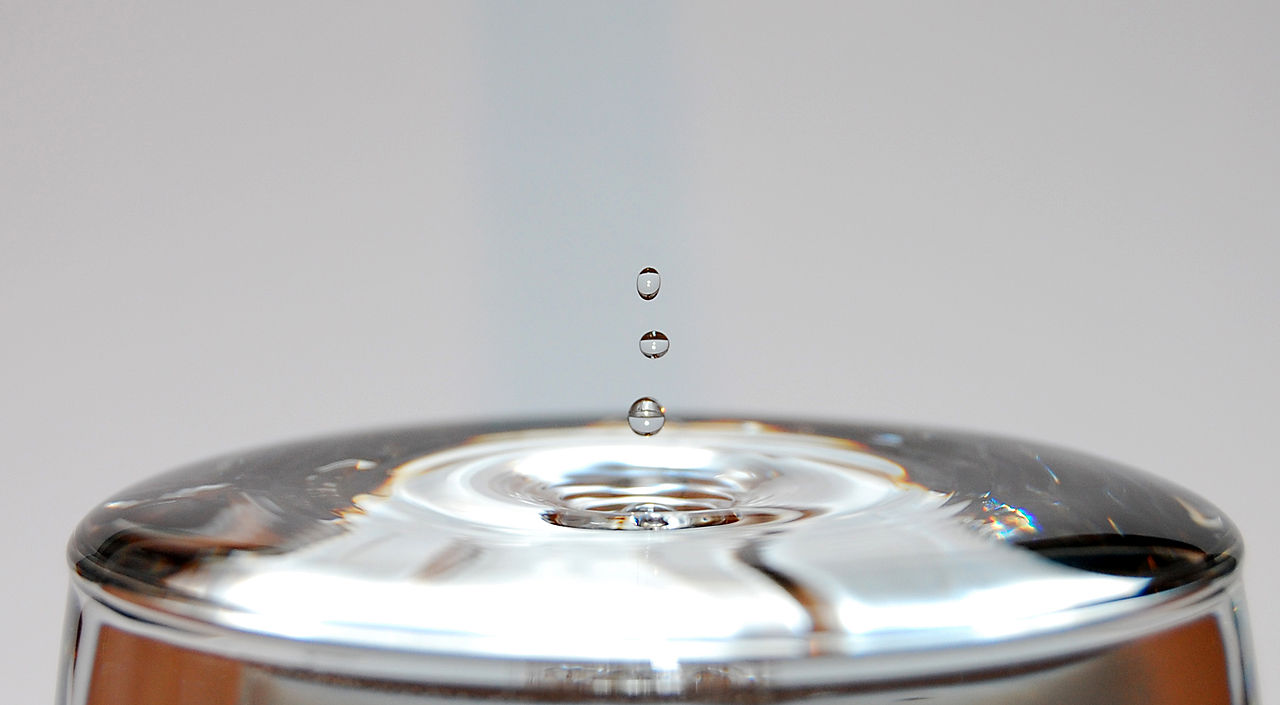
\includegraphics[width=8cm]{images/photo_liquide.jpg}
			\end{center}
			\supercaption{La tension de surface donne aux liquides des propriétés fascinantes mais sans aucune conséquence en thermodynamique. Il s’agit pour nous de «~la même eau~» qu’elle soit à l’état gazeux ou liquide.}%
				{\wcfile{Water_droplet_backjet.JPG}{Photo} \ccby par \wcu{Fcb981}}
  		\label{fig_oocestjoli}
		\end{figure}
	
	\subsection{Changements de phase}
	\index{phase, changements de}
	
		En chauffant de l’eau à pression ambiante (par exemple dans une casserole), il est facile de s’apercevoir que le passage de l’état liquide à l’état gazeux se fait avec une très grande variation de volume. Ainsi, à~\SI{1}{\bar} et~\SI{100}{\degreeCelsius} le volume spécifique de l’eau est multiplié par mille environ avant que la température puisse augmenter à nouveau.
		
		La variation brutale d’une propriété physique par rapport à une autre est nommée \vocab{changement de phase}. Dans ce chapitre nous nous concentrerons sur les deux phases : liquide et gazeuse.
		
		La notion de phase est délicate à définir\footnote{En fait, un changement de phase est bien plus facile à reconnaître qu’à définir. Nous nous contenterons de stipuler qu’à l’intérieur d’une phase, les propriétés varient continûment (condition nécessaire mais pas suffisante).} ; il existe de nombreuses phases différentes (liquide, solide, gazeuse, plasma, parmi d’autres) et leurs frontières ne sont pas toujours distinctes. Nous allons voir par exemple qu’il est possible de transformer un liquide en vapeur sans jamais observer d’ébullition ni de changement brutal de propriété.
		
		
		
	\subsection{Comment se représenter la liquéfaction et l’ébullition ?}
		
		Lorsque nous avions exploré le modèle du gaz parfait en \S\ref{ch_gaz_parfait_kezako}, nous nous étions représentés les molécules comme de très petites boules de billard en mouvement chaotique, se percutant sans jamais s’attirer (\cref{fig_gaz_boules}). En réalité, les molécules sont soumises à des forces d’attraction respectives qui affectent beaucoup leur comportement.
		
		Imaginons, pour commencer, deux très petites boules de billard attirées respectivement par une force magnétique et qui se percutent sans frottement à très grande vitesse (\cref{fig_billard_grande_vitesse}). La force d’attraction modifie leur trajectoire lorsque les boules sont très proches l’une de l’autre ; mais une fois qu’elles se sont éloignées, l’influence devient négligeable.

		
		\begin{figure}
			\begin{center}
				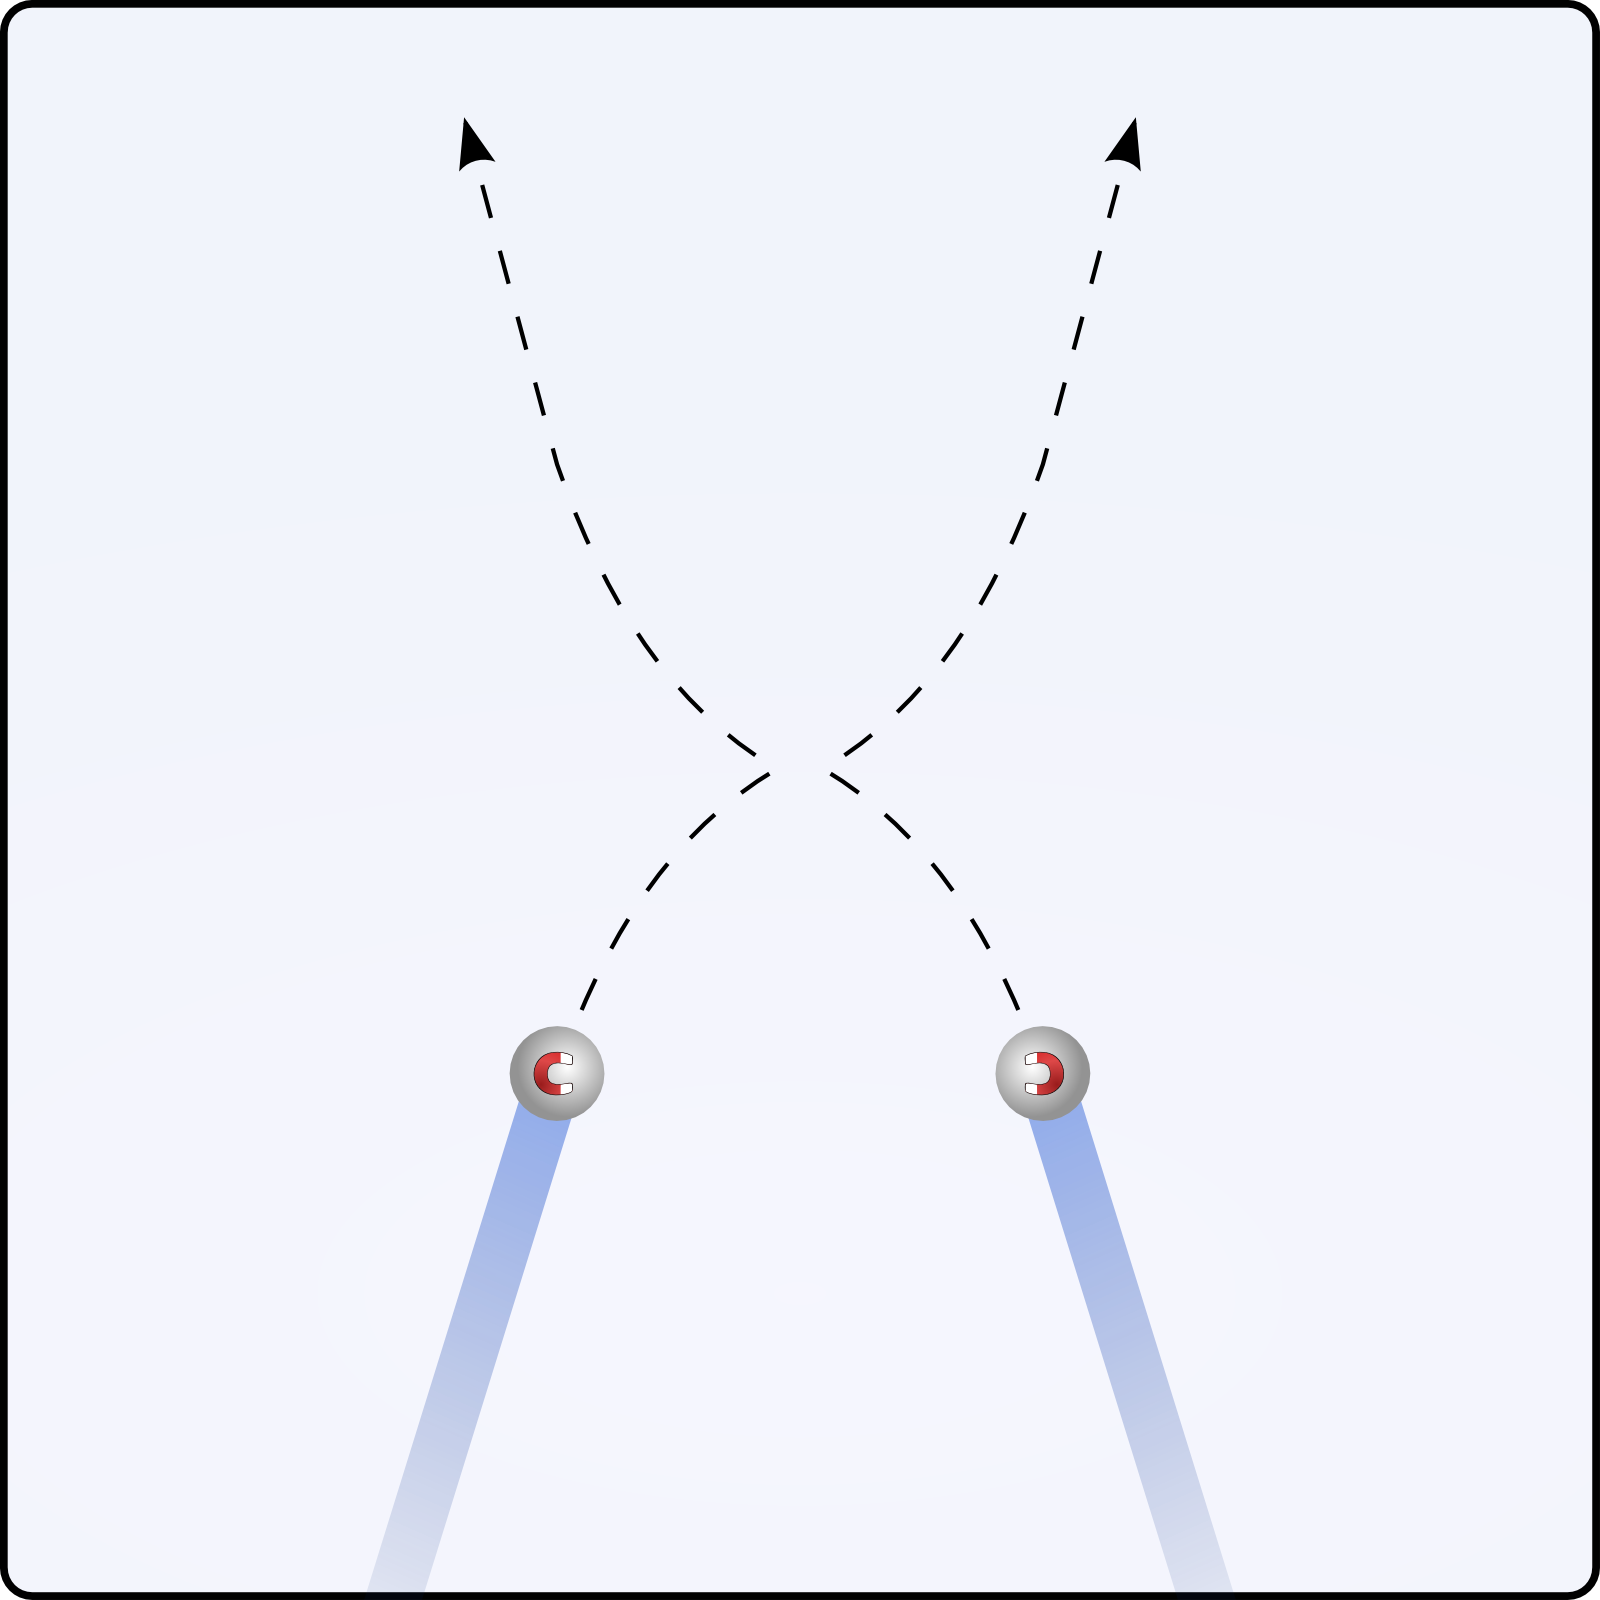
\includegraphics[width=8cm]{images/billard_rapide.png}
			\end{center}
			\supercaption{Deux boules de billard aimantées se percutant sans frottement à grande vitesse. La force d’attraction réciproque modifie la trajectoire et le comportement des deux boules, mais seulement pour un court instant et sur une courte distance.}{Schéma \ccbysa par \wcu{Sharayanan} \& \olivier}
  		\label{fig_billard_grande_vitesse}
		\end{figure}
	
		Maintenant, reproduisons l’expérience en donnant aux deux boules une vitesse plus faible (\cref{fig_billard_faible_vitesse}). En dessous d’une vitesse seuil, les boules n’auront plus assez n’énergie cinétique pour se séparer durablement. Elles formeront une paire, rebondissant périodiquement l’une contre l’autre en occupant un volume moyen nettement plus faible.
		
		\begin{figure}
			\begin{center}
				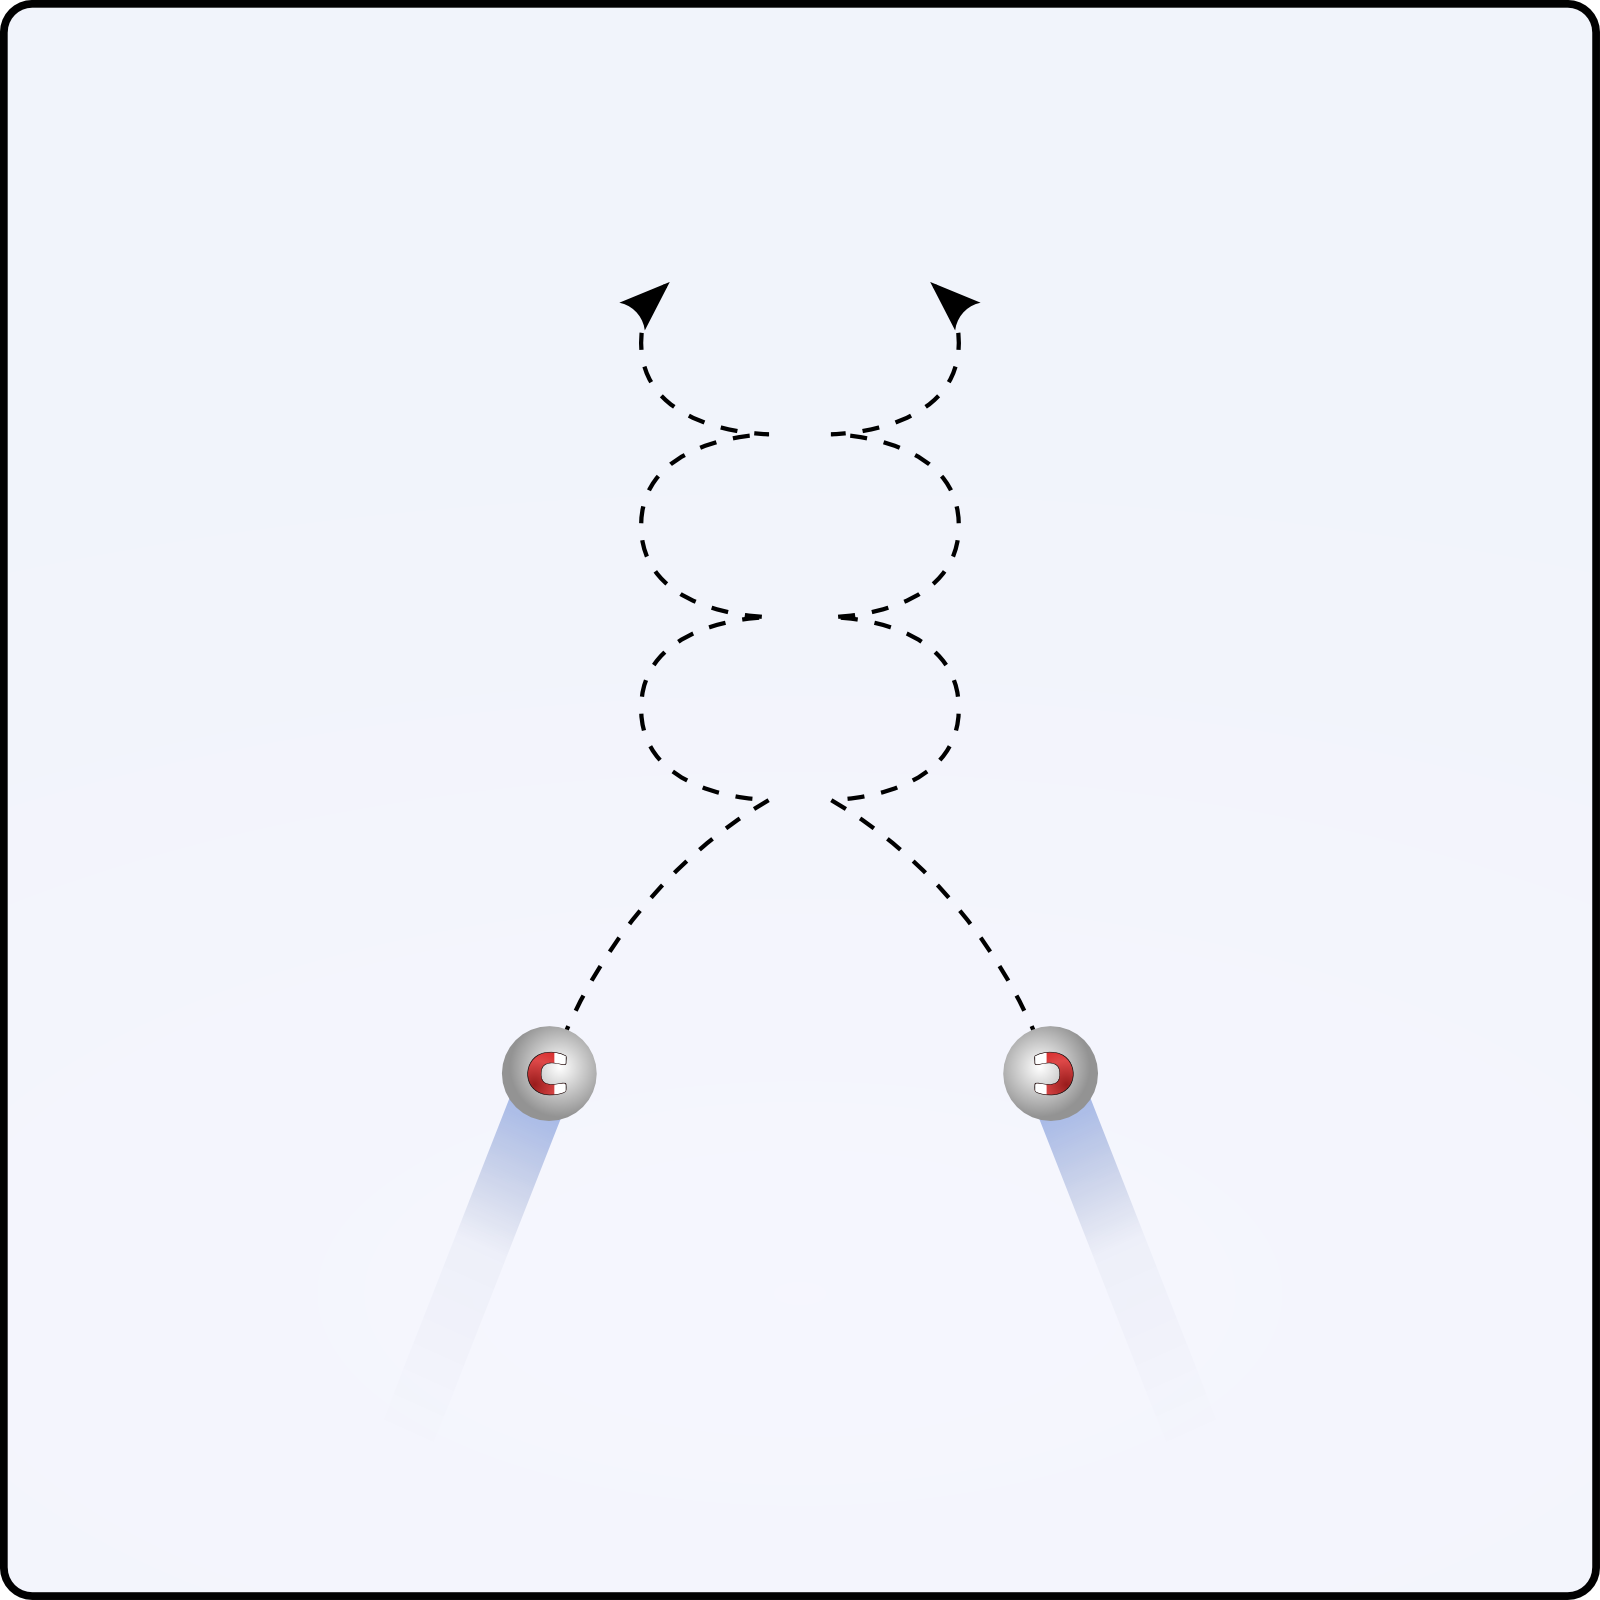
\includegraphics[width=8cm]{images/billard_lent.png}
			\end{center}
			\supercaption{Deux boules de billard aimantées se percutant sans frottement à faible vitesse. En dessous d’une vitesse seuil, les deux boules continueront leur trajectoire de façon groupée.}{Schéma \ccbysa par \wcu{Sharayanan} \& \olivier}
  		\label{fig_billard_faible_vitesse}
		\end{figure}

		Ce modèle simpliste est une bonne première approche pour décrire le phénomène de liquéfaction. Lorsque l’on réduit l’énergie cinétique des molécules d’un gaz (par refroidissement), passé un seuil critique elles s’assemblent de façon beaucoup plus compacte, tout en continuant à se percuter à la même vitesse moyenne (température inchangée). Plus l’on prélève de chaleur au gaz, plus le nombre de molécules en interaction compacte augmente. Elles forment de petits groupes ; s’ils sont suffisemment nombreux, les groupes de~\num{e14} molécules (cent mille milliards) diffusent la lumière et forment une suspension visible à l’œil nu. Dès que le nombre de molécules atteint \num{e21} l’œil humain peut identifier des gouttes de liquide.
		
		On peut ainsi liquéfier n’importe quel gaz en le refroidissant et réduisant son volume. La température et la pression à atteindre pour la liquéfaction dépendent de la taille et de la géométrie des molécules qui le composent. Dans les sections suivantes, nous allons quantifier précisément les quantités d’énergie et les gammes de propriétés nécessaires pour vaporiser et liquéfier l’eau.
	
	
	\subsection{Utilisation industrielle de l’eau et des \mbox{liquides/vapeurs}}
	
		Lorsque l’on utilise un fluide pour transformer du travail et de la chaleur, il peut être judicieux d’exploiter les phénomènes de changement de phase.

		Sous forme de vapeur, un fluide a le comportement d’un gaz et occupe spontanément tout le volume qui lui est accordé. On l’utilise souvent sous cette forme pour déplacer des pièces mécaniques (piston dans un cylindre, pales de turbine).
		
		Sous forme liquide, le fluide a une densité très nettement supérieure. On l’utilise souvent sous cette forme pour transférer de la chaleur (réchauffement ou refroidissement) car la taille des conduits peut être très faible. Par exemple, un radiateur rempli d’air ou de vapeur devrait être environ mille fois plus grand qu’un radiateur empli de liquide pour avoir la même puissance.
		
		Historiquement, l’eau a été utilisée dans les tout premiers moteurs de l’histoire pour ces raisons et parce que les variations de volume lors des changements de phase permettent un contrôle plus aisé des machines avec une technologie faible. De nos jours, les liquides/vapeurs sont surtout utilisés dans deux grands types d’applications :
			\begin{description}
				\item [Dans les centrales électriques] où les liquides/vapeurs permettent un prélèvement de chaleur efficace depuis des sources externes (combustion de déchets, réactions nucléaires, géothermie). On y utilise de l’eau, liquide abondant même s’il doit être purifié pour éviter les dépôts calcaires. Le \coursneuf est tout entier dédié à ces machines.
				\item [Dans les réfrigérateurs] où les liquides/vapeurs permettent l’utilisation de composants compacts, notamment les pompes\footnote{L’utilisation des liquides/vapeurs permet aussi de faire chuter la température du fluide sans utiliser de pièce mobile (une simple soupape suffit), ce qu’un gaz parfait ne permet pas (\S\ref{ch_principe_de_joule}).}. On y utilise une variété de fluides (dits alors «~frigorigènes~» même s’ils n’ont rien d’extraordinaire) choisis en fonction de leur plage de propriétés, leur coût, leur influence sur la couche d’ozone et leur contribution au réchauffement climatique.
			\end{description}

		Nous nous concentrons ici sur l’eau, mais les phénomènes décrits et les méthodes de calcul s’appliquent tout aussi bien aux autres liquides/vapeurs.



\section{Description qualitative des propriétés de l’eau}


	\subsection{Les limites du gaz parfait}

		\thermoquotebegin{O}
		Les gaz font preuve dans leur comportement, en particulier dans les relations de volume, température et de pression exprimées par les lois de Mariotte et Gay-lussac, de tant de régularité qu’ils nous amènent à la notion que l’attraction mutuelle des particules, qui a lieu dans les corps solides et fluides, est annulée dans leur cas ; de sorte que bien qu’avec les solides et liquides la chaleur nécessaire à provoquer une expansion doit surmonter une résistance interne et une résistance externe, seule la seconde a un effet dans le cas des gaz.
		\thermoquoteend{Rudolf Clausius, 1850~\mbox{\cite{clausius1850, clausius1850en, clausius1868fr1}}}{\vspace{3em}} %handmade vspace
		
		Au fur et à mesure que l’on ralentit et rapproche les molécules d’un gaz les unes des autres, le modèle du gaz parfait décrit de plus en plus mal ses propriétés. On observe un seuil en dessous duquel on observe la liquéfaction et l’ébullition, c’est-à-dire la coexistence des deux phases liquide et gazeuse ; ce seuil est décrit en termes de température et de pression qui sont dites \vocab[critiques, pression et température]{critiques}\index{température!critique}\index{pression!critique}. Les températures et pressions critiques de quelques fluides courants sont indiquées dans le \cref{tab_exemples_températures_pressions_critiques}. Notons que l’air, mélange de plusieurs gaz, verra différentes substances de sa composition se condenser à différentes températures.

		\begin{table}
			\begin{center}
			\begin{tabularx}{10cm}{l l S S}
			~  			& ~  		& {$T_\text{cr.}$ (\si{\kelvin})} 	& {$p_\text{cr.}$ (\si{\mega\pascal})}	\\
			\hline
			Air 			& --  		& 132 				& 3,8		\\
			Chlore 		& $Cl_2$		& 417 				& 7,71		\\
			Dioxyde de carbone 	& $CO_2$ 	& 304,2	& 7,39		\\
			Eau 			& $H_20$ 	& 647,1 				& 22,06		\\
			Hélium 		& $He$		& 5,3 				& 0,23		\\
			Oxygène 		& $O_2$		& 154,8				& 5,08		\\
			R-134a 		& $CF_{3}CH_2F$ & 374,2			& 4,059		\\
			Xénon 		& $Xe$ 		& 289,8				& 5,88		\\
			\end{tabularx}
			\end{center}
		\caption{Température et pression critiques de quelques substances.
			En pratique, dans l’industrie, l’ingénieur/e fera surtout usage des propriétés de deux corps : l’eau (dans les moteurs à vapeur) et le réfrigérant R-134a (dans les thermopompes et réfrigérateurs). Dans ce chapitre, nous n’utiliserons que l’eau, mais les principes restent identiques pour tous les corps.}
			\label{tab_exemples_températures_pressions_critiques}
		\end{table}
	

		Lorsqu’on le maintient à une température et une pression nettement supérieures à ses valeurs critiques, un fluide se comporte comme un gaz parfait. Tous les fluides que nous assimilons traditionnellement à des liquides (par exemple, le mercure) ou des gaz (par exemple, le $CO_2$) peuvent passer d’un état à l’autre.


	\subsection{Le diagramme température-volume ($T$-$v$)}
	\label{ch_lv_diagramme_tv}

		Observons la température et le volume d’une masse d’eau pure que l’on chauffe continûment, alors qu’elle est placée dans un récipient à pression constante (\cref{fig_changement_phase}). On mesure alors la température de l’eau en fonction de son volume (\cref{fig_T-v_construction_1}).

		\begin{figure}
			\begin{center}
				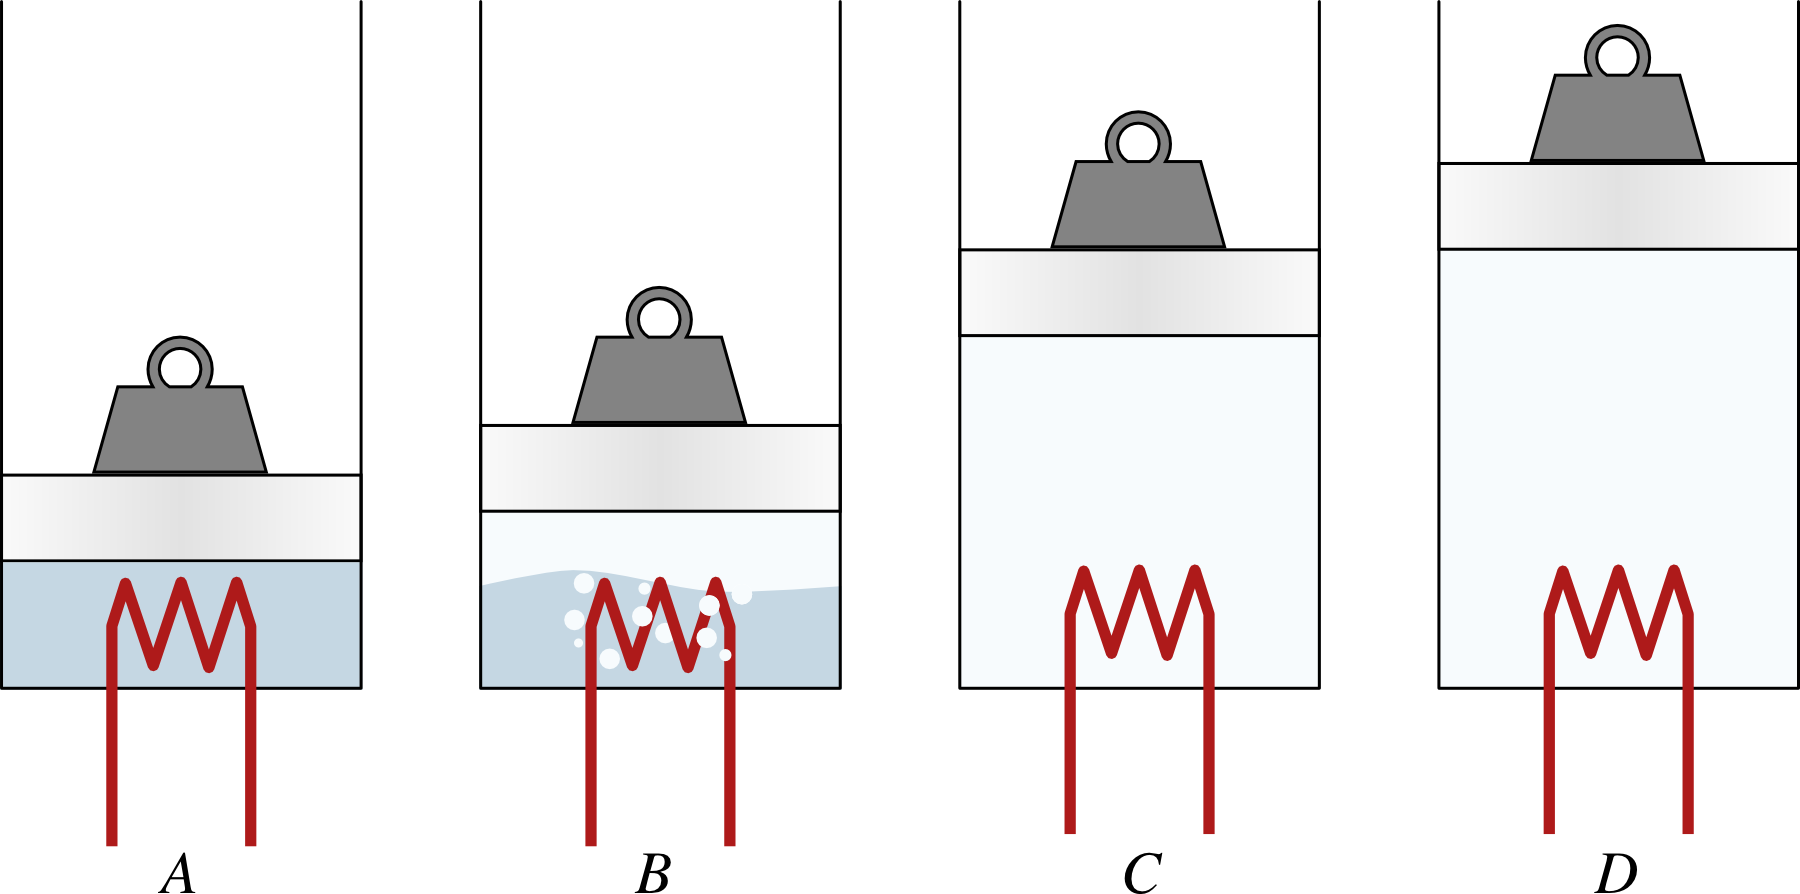
\includegraphics[width=\textwidth]{images/etats_vapeur_pression_constante.png}
			\end{center}
			\supercaption{Réchauffement d’une quantité fixe d’eau à pression constante.\\
				A : liquide comprimé ; B : mélange liquide-vapeur ; C : vapeur saturée ; D : vapeur sèche.}{\cczero \oc}
			\label{fig_changement_phase}
		\end{figure}

		\begin{figure}
			\begin{center}
				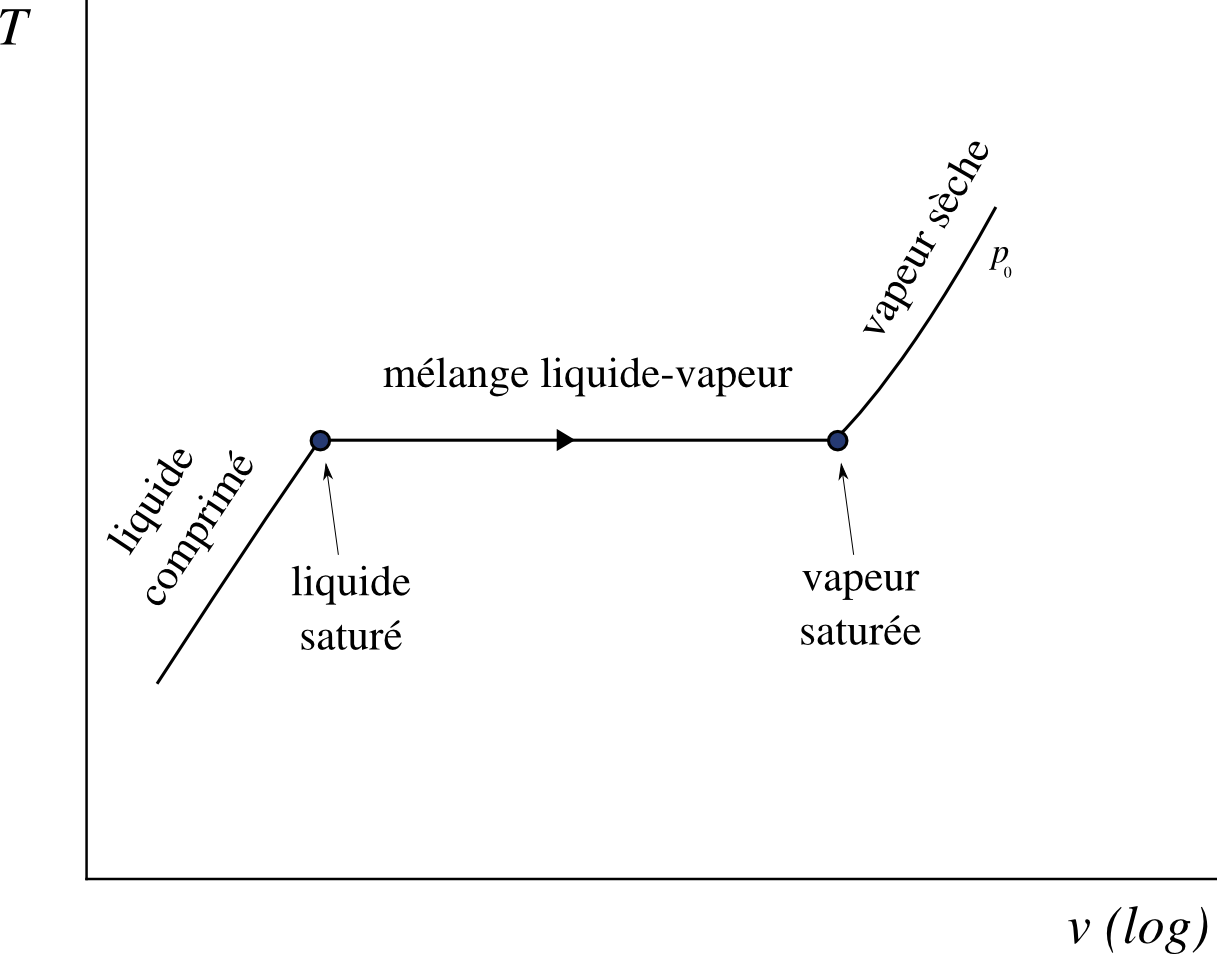
\includegraphics[width=\didacticpvdiagramwidth]{images/etats_vapeur_t_v.png}
			\end{center}
			\supercaption{Vocabulaire : état de l’eau pendant une évolution à pression constante.}{\cczero \oc}
			\label{fig_T-v_construction_1}
		\end{figure}

		Au départ, lorsque l’eau est liquide, la température augmente linéairement avec le volume, avec un fort gradient. On parle alors de \vocab[liquide!comprimé]{liquide comprimé}\footnote{Liquide comprimé ou \vocab[liquide!sous-refroidi]{sous-refroidi}}.\index{comprimé, liquide}\index{sous-refroidi, liquide} % en anglais : \vocabe{unsaturated}, \vocabe{compressed} or \vocabe{subcooled liquid})

		\thermoquotebegin{O}
		La vapeur peut être considérée à l’instant même de sa formation dans la chaudière, et encore en contact avec le liquide dont elle émane, ou bien séparée de ce même liquide ; et selon chacun de ces cas, ses propriétés sont différentes.
		\thermoquoteend{François-Marie Guyonneau de~Pambour, 1839}{\textit{Théorie de la machine à vapeur}~\cite{pambour1839}\vspace{-1em}}%handmade

		Puis, soudainement, alors que le volume continue de croître, la température cesse d’augmenter. Le mélange dans le cylindre est alors di-phasique : une partie est liquide, et l’autre gazeuse. L’ajout de chaleur ne provoque aucune augmentation de température (contrairement à un gaz parfait), mais seulement la transformation de liquide en vapeur : c’est l’ébullition.

		Dans cet état, la substance est appelée \vocab{mélange liquide-vapeur}\index{liquide-vapeur, mélange}\footnote{Rigoureusement, le mélange est nommé \vocab{mélange liquide-vapeur saturé}\index{saturé, mélange liquide-vapeur}, puisqu’il est composé de \vocab[liquide!saturé]{liquide saturé}\index{saturé, liquide} (parfois dit \vocab[liquide!saturant]{saturant}\index{saturant, liquide}) et de \vocab[vapeur!saturée]{vapeur saturée}\index{saturée, vapeur} (parfois dite \vocab[vapeur!saturante]{saturante}\index{saturante, vapeur}). En anglais : \vocabe{wet vapour}.}\nolinebreak.

		Enfin, lorsque la dernière goutte de liquide a été transformée en vapeur, la température reprend son augmentation au fur et à mesure que l’on apporte de la chaleur. Le fluide est alors dans un état dit de \vocab[vapeur!sèche]{vapeur sèche}\footnote{\vocab[vapeur!sèche]{Vapeur sèche} ou \vocab[vapeur!surchauffée]{surchauffée}\index{surchauffée, vapeur}.}\nolinebreak.%(en anglais : \vocabe{superheated} ou \vocabe{dry vapour})

		\clearfloats %handmade
		\thermoquotetopbegin{O}%handmade
		L’eau ne pouvant se vaporiser sous une haute pression qu’en vertu d’une température plus élevée, on a lieu de penser que, toutes circonstances égales d’ailleurs, la machine doit être capable de vaporiser moins d’eau sous une pression plus considérable.
		\thermoquoteend{François-Marie Guyonneau de~Pambour, 1835}{\textit{Traité théorique et pratique des machines locomotives}~\cite{pambour1835}\vspace{4em}} %handmade vspace
		L’expérience peut être renouvelée à des pressions différentes (\cref{fig_T-v_construction_2}). Lorsque la pression que l’on impose augmente, on observe deux faits importants :
		\begin{itemize}
			\item La température de changement de phase augmente ;
			\item La plage de volume parcourue pendant le changement de phase diminue.
		\end{itemize}

		\begin{figure}
			\begin{center}
				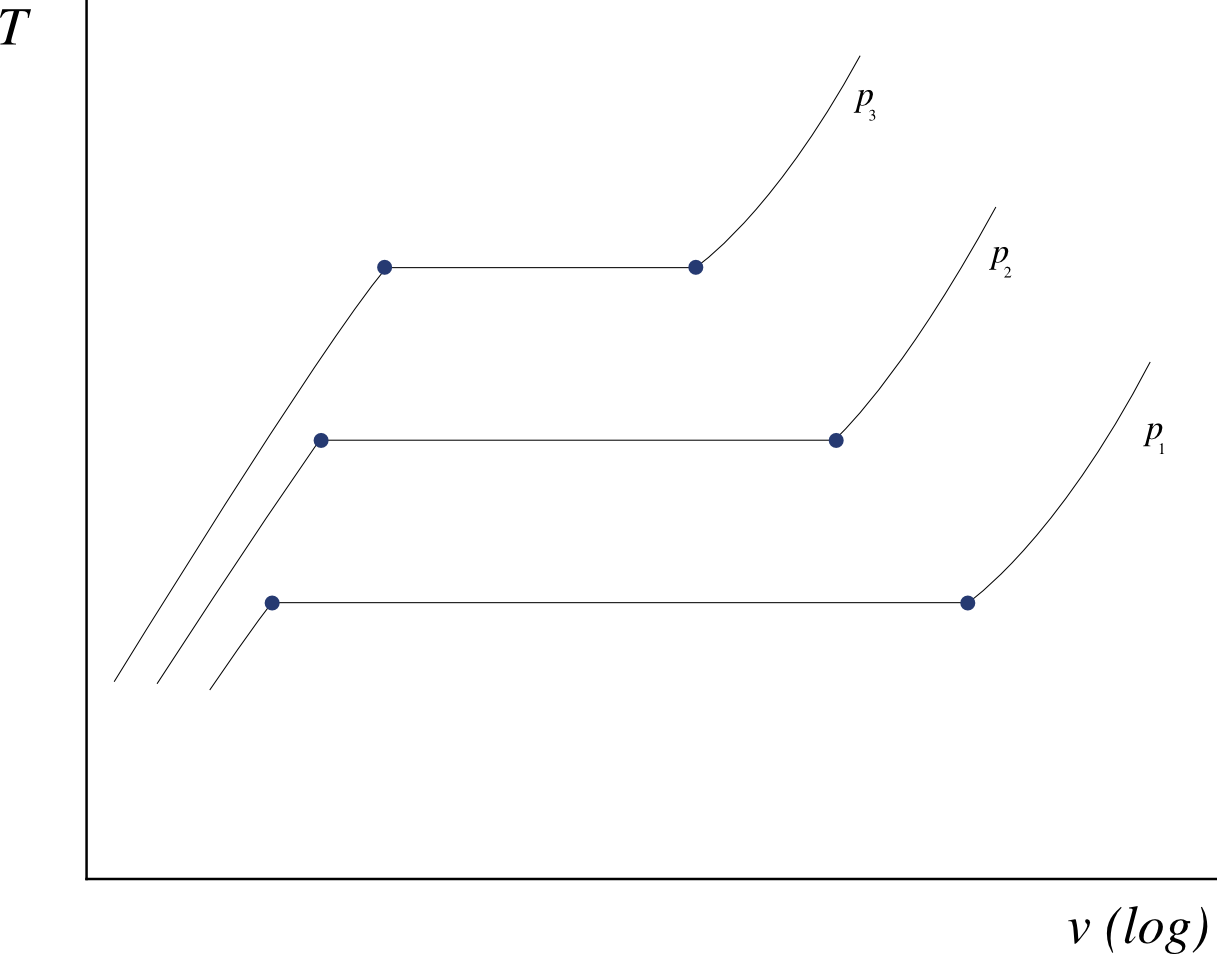
\includegraphics[width=\didacticpvdiagramwidth]{images/tv_liquidevapeur_construction.png}
			\end{center}
			\supercaption{Propriétés de l’eau tracées sur un diagramme température-volume, lorsque l’on effectue l’expérience décrite en \cref{fig_changement_phase} à différentes pressions. On observe que plus la pression est grande, plus la plage d’ébullition est petite.}{\cczero \oc}
			\label{fig_T-v_construction_2}
		\end{figure}

		Au-dessus d’une certaine pression nommée \vocab[pression!critique]{pression critique}\index{critique, pression} $p_\text{cr.}$, le changement de phase se fait de façon indistincte et il n’y a plus de plage de température constante. Le liquide devient vapeur sans bouillir !

		Au final, on peut relier entre eux tous les points de changement de phase, à toutes les pressions différentes : on obtient une courbe nommée \vocab[courbe!de saturation]{courbe de saturation}\index{saturation, courbe de}\footnote{La courbe de saturation est parfois divisée arbitrairement en deux parties nommées \vocab[courbe!de rosée]{courbe de rosée}\index{rosée, courbe de} à droite et \vocab[courbe!d’ébullition]{courbe d’ébullition}\index{ébullition, courbe d’} à gauche.}. Toutes ces informations peuvent être regroupées sur un diagramme température-volume ($T$-$v$) représenté en \cref{fig_t-v_eau}, qui décrit bien les propriétés des mélanges liquide-vapeur. L’étudiant/e est encouragé/e à s’entraîner à le reproduire.

		\begin{figure}
			\begin{center}
				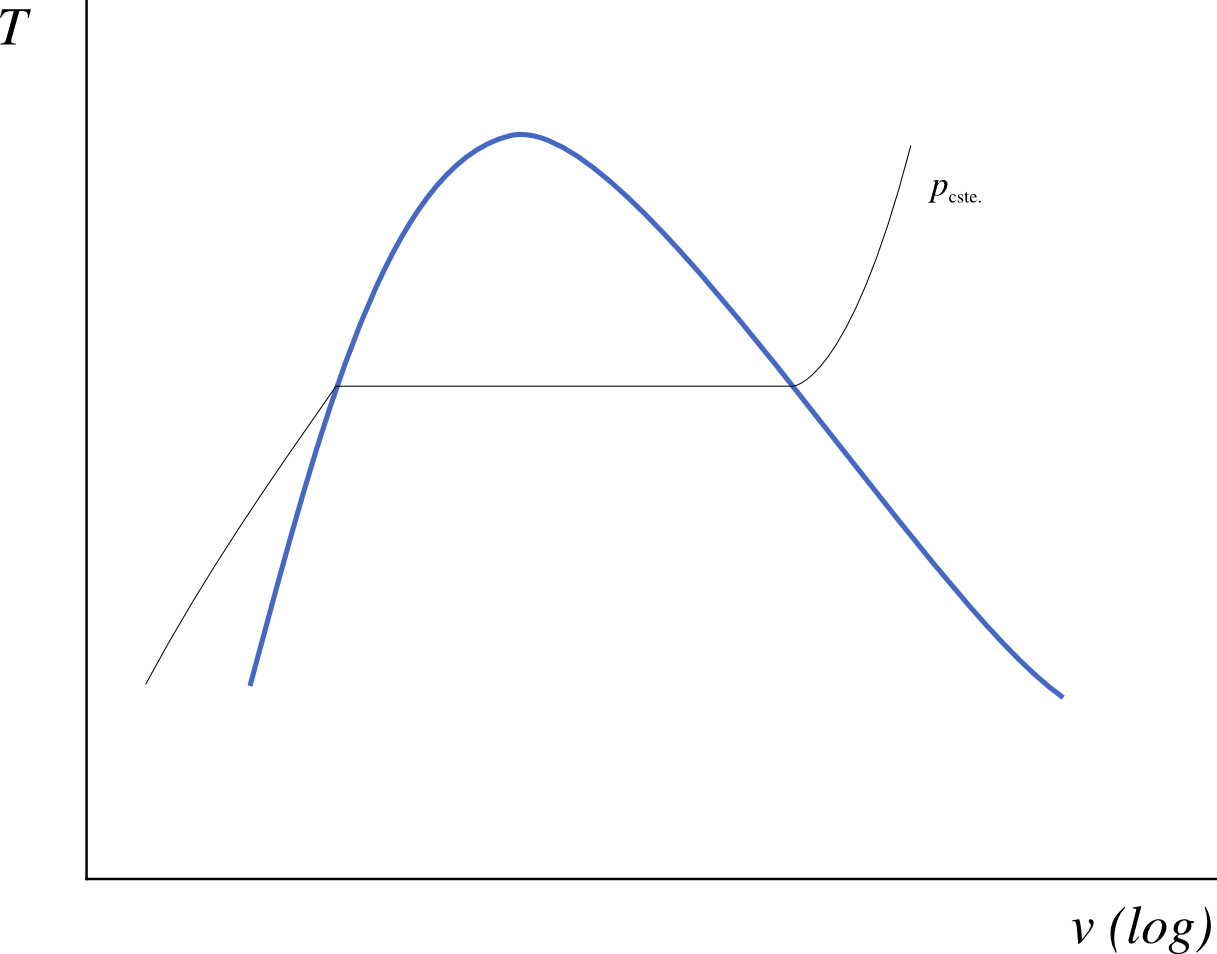
\includegraphics[width=\didacticpvdiagramwidth]{images/tv_liquidevapeur.png}
			\end{center}
			\supercaption{Diagramme température-volume de l’eau, représenté avec une évolution à pression constante (isobare). La courbe de saturation est représentée en bleu.}{\cczero \oc}
			\label{fig_t-v_eau}
		\end{figure}


	\subsection{Le diagramme pression-volume ($p$-$v$)}
	\label{ch_lv_bain_marie}

		Pour bien cerner le phénomène de changement de phase, imaginons maintenant une expérience légèrement différente.
		
		On se propose de faire varier le volume d’une masse donnée d’eau, en maintenant sa température constante (par exemple en plongeant le récipient dans un bain-marie). On observe alors la pression à l’intérieur du récipient (\cref{fig_p-v_construction_1}).
		
		Tant que l’eau est liquide, on observe que la pression chute très fortement au fur et à mesure que l’on augmente son volume. Puis, soudainement, la pression reste parfaitement constante, alors que volume continue d’augmenter : à l’intérieur du cylindre, l’eau se met à bouillir et on a un mélange liquide-vapeur. Enfin, lorsque la dernière goutte d’eau liquide s’est évaporée, la pression reprend sa décroissance.

		\begin{figure}
			\begin{center}
				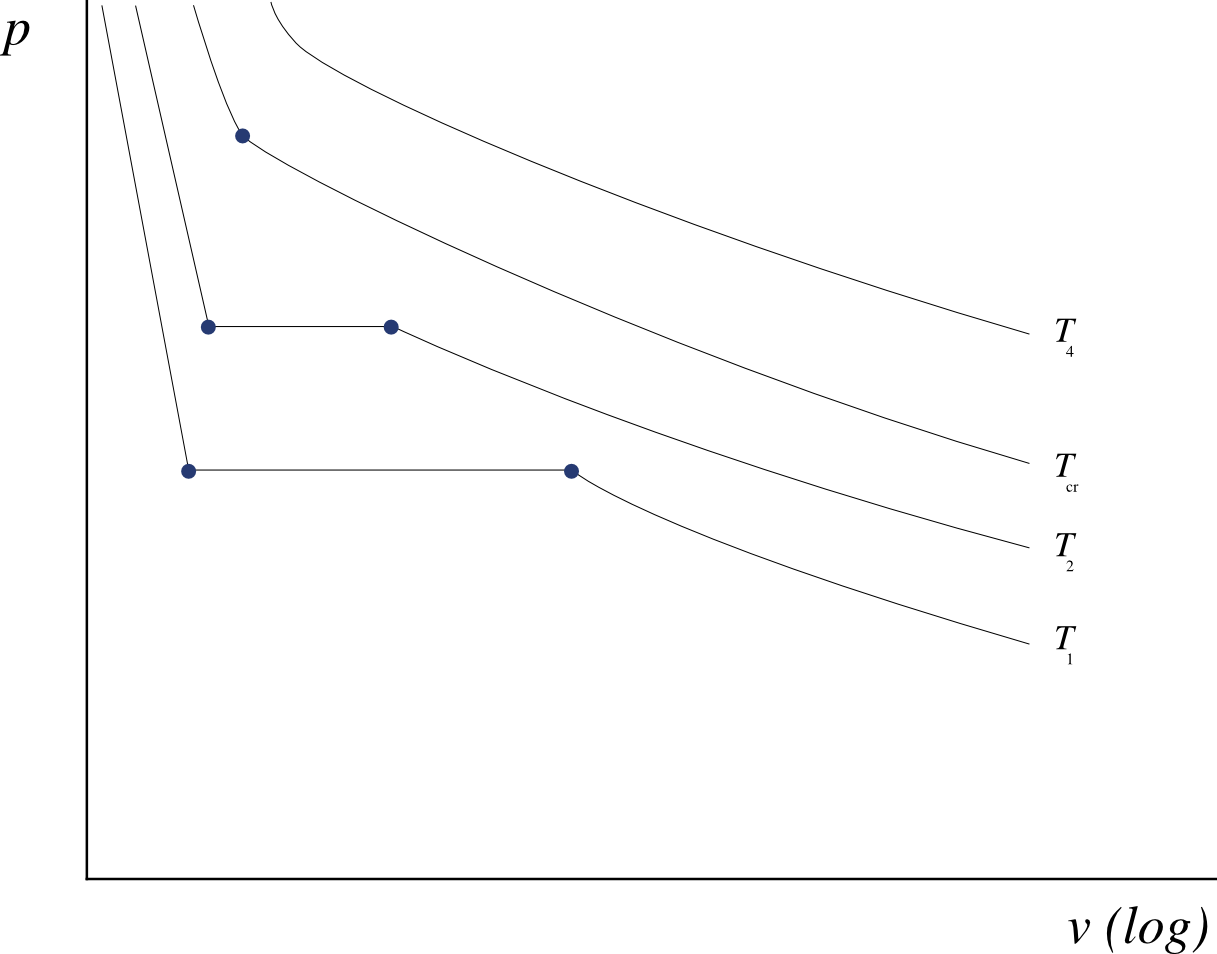
\includegraphics[width=\didacticpvdiagramwidth]{images/pv_liquidevapeur_construction.png}
			\end{center}
			\supercaption{Propriétés de l’eau tracées sur un diagramme pression-volume, lorsque l’on maintient la température constante en faisant varier le volume.}{\cczero \oc}
			\label{fig_p-v_construction_1}
		\end{figure}

		\thermoquotebegin{O}
		Lorsque la vapeur, après avoir été formée dans une chaudière, continue d’être en contact avec son eau de génération, on observe que la même température correspond invariablement à la même pression et réciproquement. Il est alors impossible d’augmenter sa température, sans qu’aussitôt sa pression et sa densité augmentent spontanément.
		\thermoquoteend{François-Marie Guyonneau de~Pambour, 1839}{\textit{Théorie de la machine à vapeur}~\cite{pambour1839}}
		
		Si l’on reproduit l’expérience à différentes températures, on constate que plus la température est haute, plus la plage de changement de phase est courte. Au-dessus d’une température, dite critique ($T_\text{cr.}$), la plage disparaît tout à fait.

		Le comportement d’un liquide-vapeur peut être ainsi décrit sur un diagramme pression-volume ($p-v$) comme montré en \cref{fig_p-v_eau}. L’étudiant/e est également encouragé/e à reconstruire ce schéma.

		\begin{figure}
			\begin{center}
				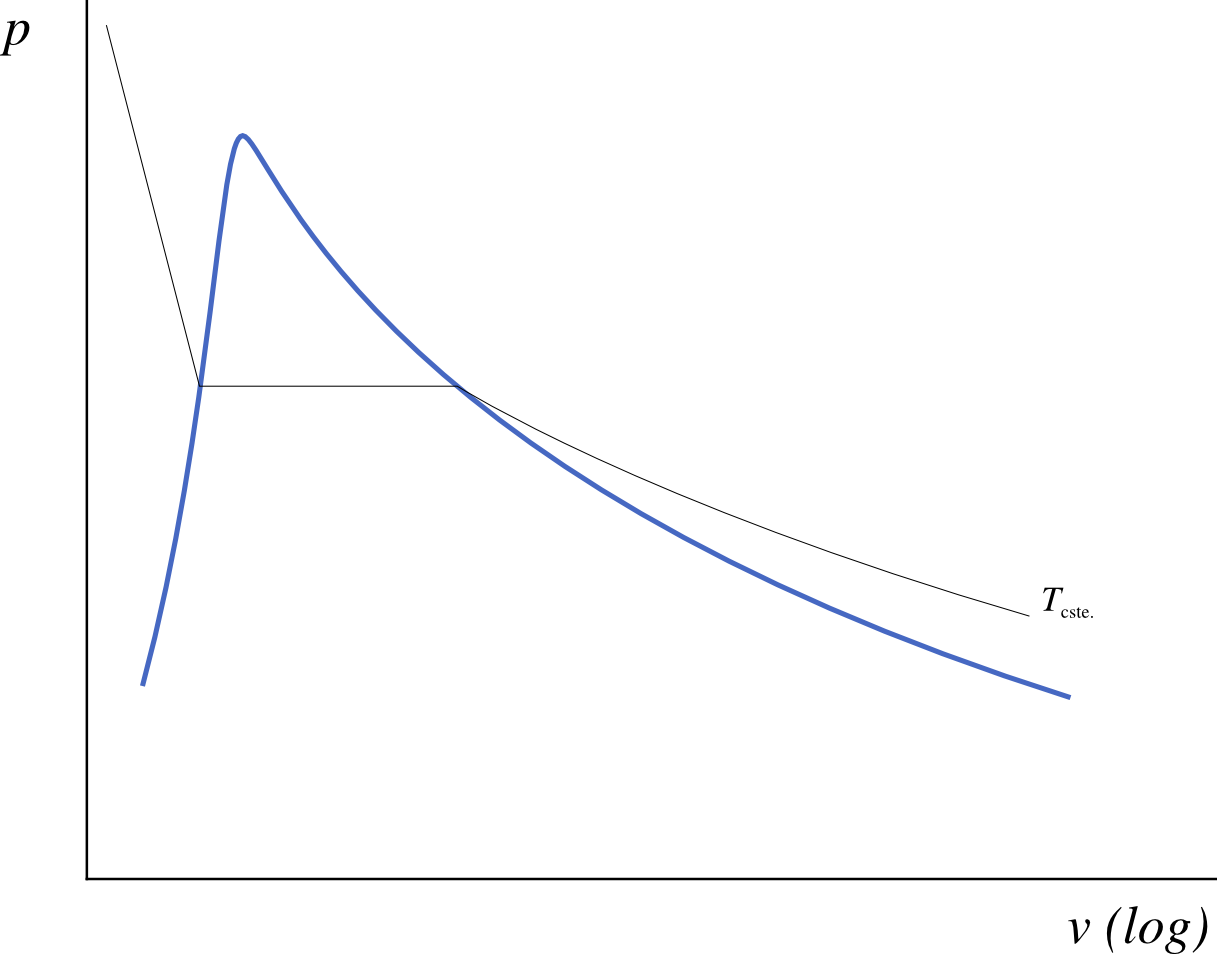
\includegraphics[width=\didacticpvdiagramwidth]{images/pv_liquidevapeur.png}
			\end{center}
			\supercaption{Diagramme pression-volume de l’eau, représenté avec une évolution à température constante (isotherme). La courbe de saturation est représentée en bleu.}{\cczero \oc}
			\label{fig_p-v_eau}
		\end{figure}

	
			
	\subsection{Pièges pour l’étudiant/e}
	
		La notion la plus importante à retenir du comportement des liquides-vapeurs est que contrairement aux gaz parfaits, \emph{la température y est complètement déréglée}. Elle ne dicte plus simplement les autres propriétés.
		
		Insistons bien. Pour un fluide proche d’un changement de phase :
			\begin{IEEEeqnarray}{rCl}
				p v 	& \not\propto 	& T \\
				u 		& \not\propto 	& T \\
				h 		& \not\propto 	& T							
			\end{IEEEeqnarray}
	
		Presque tout ce qui a été vu au \coursquatre doit être oublié lorsque l’on utilise un liquide/vapeur. Heureusement, les trois premiers chapitres n’ont rien perdu de leur utilité.



	\subsection{L’eau dans la vie courante}
	
		Les phénomènes que nous décrivons ici sont facilement observables et reproductibles avec de l’eau dans la vie courante. Toutefois, il faut noter que :
			
			\begin{itemize}
				\item La vapeur d’eau est transparente et quasiment invisible. Ce que l’on observe au-dessus d’une casserole d’eau en ébullition ou sous la forme de nuages est de l’eau \emph{liquide} en suspension dans l’air (\cref{fig_tazaazul}). Ces fines gouttelettes liquides peuvent s’assembler pour former des gouttes\footnote{Au fur et à mesure qu’une gouttelette croît, la surface offrant une résistance par frottement augmente moins vite que son poids ; elle finit par chuter.} ou bien s’évaporer à nouveau et redevenir ainsi invisible.
				
			\begin{figure}
				\begin{center}
					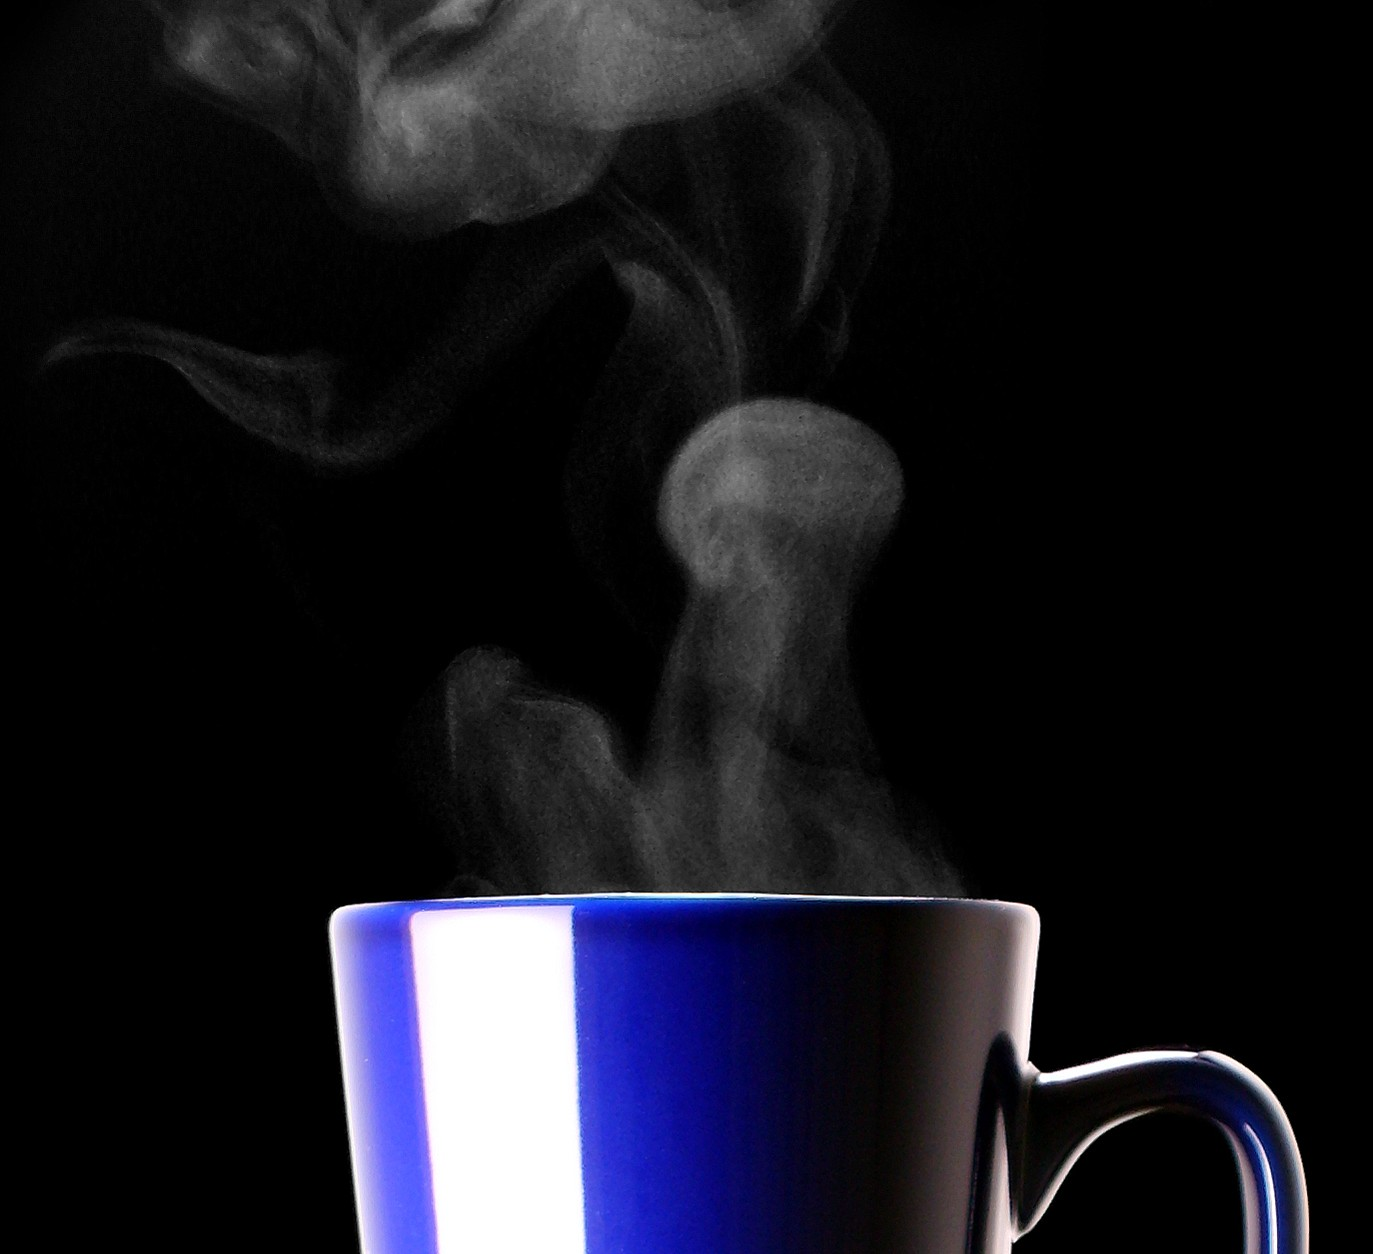
\includegraphics[width=6cm]{images/taza_azul.jpg}
				\end{center}
				\supercaption{L’eau visible au-dessus d’un récipient de liquide chaud, parfois nommée \vocab{buée}, est à l’état liquide et non gazeux. Ces gouttelettes sont observables à l’œil nu.}{Photo \pd \wcfile{Taza_azul.jpg}{par Jorge Barrios} (recadrée)}
				\label{fig_tazaazul}
			\end{figure}
				
				\item L’air est partiellement constitué de vapeur d’eau (et sa capacité massique à porter de l’eau augmente avec la température). Lorsque l’on fait bouillir de l’eau liquide à l’air libre, il ne faut pas oublier que c’est l’air qui accueille la vapeur d’eau ; l’ébullition se déroule donc assez différemment de l’expérience décrite en \cref{fig_changement_phase}\footnote{On peut noter, par exemple, que la température de l’eau liquide chute sensiblement lors d’une évaporation à pression constante dans l’air. Autre différence, la condensation est catalysée par la présence de particules de poussière dans l’air.}\nolinebreak.
			\end{itemize}





\section{Quantification des propriétés de l’eau}

		\thermoquotebegin{O}
			Aussi voyons-nous que des mathématiciens très distingués ont proposé, sur le mouvement du piston dans les machines à vapeur, des formules analytiques qui seraient très vraies, si effectivement les choses se passaient dans la machine comme ils le supposent ; mais qui, faute d’un point de départ vrai dans le calcul, tombent d’elles-mêmes en présence des faits. De là résulte encore que dans la pratique les proportions de ces machines n’ont été déterminées que par des essais multipliés, et que l’art de les construire ne procède encore que par tâtonnement et par imitation.
		\thermoquoteend{François-Marie Guyonneau de~Pambour, 1835}{\textit{Traité théorique et pratique des machines locomotives}~\cite{pambour1835}}
	Pour un liquide/vapeur, il n’existe pas de moyen simple de quantifier l’énergie interne~$u$ et l’enthalpie~$h$ qui nous intéressent tant. En effet, à partir de $p$ et $v$, on ne peut pas calculer la température ($p v \not\propto T$) et à partir de $T$, on ne peut pas calculer $u$ et $h$ ($u \not\propto T$ et $h \not\propto T$).
	
	\begin{itemize}
		\item La mauvaise nouvelle est qu’il va nous falloir, pour cela, utiliser des tableaux de propriétés déjà mesurées, nommés \vocab{abaques de vapeur}\index{vapeur!abaques de}, ce qui est parfois fastidieux ;
		\item La bonne nouvelle est que ces abaques nous dispensent des effroyables relations mathématiques (du type $(T_1/T_2)^{1/\gamma-1} = \ldots$) qui décrivaient les propriétés des fluides au \coursquatre.
	\end{itemize}

	\subsection{Liquide comprimé et vapeur sèche}
 		
		Commençons par chauffer une quantité fixe d’eau liquide en maintenant sa pression constante, comme nous l’avons fait en \cref{fig_changement_phase}. Pour chaque température, nous mesurons $v$, $u$, et $h$\footnote{Ainsi que $s$, mais c’est une surprise que nous gardons pour le \courshuitshort…}. L’expérience est ensuite reconduite pour une pression différente.
		
		L’ensemble des mesures est tabulé dans l’abaque~n°1, dont un extrait est présenté en \cref{tab_abaque1extrait}.
		
		\begin{table}
		\begin{center}
		\begin{footnotesize}
		\begin{tabular}{
		|S[table-format = 4.0]|%				T
		S[table-format = 2.6]% 		v
		S[table-format = 4.1]%			u
		S[table-format = 4.1]%		h
		S[table-format = 2.4]|%	s
		}

 		\hline
		%\addlinespace[10pt]
		 &&&&\\
		\multicolumn{1}{|@{}c@{}|}{{\scriptsize °C}}	% Using SIunit screws the table up here for some reason
		&\multicolumn{1}{@{}c@{}}{{\small\si[per-mode = fraction]{\metre\cubed\per\kilogram}}}%
		&\multicolumn{1}{@{}c@{}}{{\small\si[per-mode = fraction]{\kilo\joule\per\kilogram}}}%
		&\multicolumn{1}{@{}c@{}}{{\small\si[per-mode = fraction]{\kilo\joule\per\kilogram}}}%
		&\multicolumn{1}{@{}c@{}|}{{\small\si[per-mode = fraction]{\kilo\joule\per\kilogram\per\kelvin}}}\\%

		%\addlinespace[10pt]
		 &&&&\\
		{$T$}	&$v$	&$u$	&$h$	&$s$\\
		\hline
 		
		&\multicolumn{4}{c|}{$p = \SI{1,6}{\mega\pascal}$}\\
		&\multicolumn{4}{c|}{($T_\text{sat} = \SI{201,37}{\degreeCelsius}$)}\\
		
		10		&0,001		&42		&43,6		&0,1509\\
		20		&0,001001	&83,8		&85,4		&0,2962\\
		50		&0,001011	&209,1	&210,7	&0,7031\\
		100	&0,001043	&418,6	&420,3	&1,306\\
		200	&0,001156	&850,4	&852,3	&2,3305\\	\cdashline{2-5}[.8pt/2pt]
		300	&0,15866	&2781,5	&3035,4	&6,8863\\
		500	&0,22029	&3120,1	&3472,6	&7,5409\\
		600	&0,24999	&3293,9	&3693,9	&7,81\\
		700	&0,2794	&3473,5	&3920,5	&8,0557\\
		800	&0,30865	&3659,5	&4153,3	&8,2834\\
		900	&0,3378	&3852,1	&4392,6	&8,4965\\
		1000	&0,36687	&4051,2	&4638,2	&8,6974\\
		1100	&0,39589	&4256,6	&4890		&8,8878\\
		1200	&0,42487	&4467,9	&5147,7	&9,0689\\
		1500	&0,51169	&5133,7	&5952,4	&9,5656\\
		2000	&0,65615	&6326,8	&7376,6	&10,272\\
		\hline

 		\end{tabular}\end{footnotesize}\end{center}
 		\caption{Extrait de l’abaque~n°1. Ici les mesures sont faites à~\SI{1,6}{\mega\pascal}, c’est-à-dire \SI{16}{\bar}. On observe une discontinuité entre \SI{200}{\degreeCelsius} et~\SI{300}{\degreeCelsius} : c’est le changement d’état qui a eu lieu à $T_\text{sat} = \SI{201,37}{\degreeCelsius}$.}
 		\label{tab_abaque1extrait}
 		\end{table}

		\clearfloats %handmade
		Cet abaque~nous permet de répondre à de nombreuses questions. Quelques exemples :
			
			\begin{anexample}
			À \SI{16}{\bar} et~\SI{600}{\degreeCelsius}, quel volume occupent \SI{2}{\kilogram} d’eau ?
			
				\begin{answer}La pression est de~\SI{1,6}{\mega\pascal}. Dans l’abaque~n°1, pour cette pression, à~\SI{600}{\degreeCelsius}, on peut lire son volume spécifique à $v = \SI{0,24999}{\metre\cubed\per\kilogram}$. Le volume total sera donc de $V = m \ v = \SI{0,49998}{\metre\cubed}$, que nous arrondissons sans hésiter à~\SI{0,5}{\metre\cubed}.
					\begin{remark}On remarque que la température est supérieure à la température de saturation (\SI{201,37}{\degreeCelsius}), l’eau sera donc à l’état de vapeur sèche.\end{remark}
					\begin{remark}Avec un gaz parfait, nous pouvions simplement \emph{calculer} le résultat ($v = \frac{R T}{p}$) ; mais cela ne fonctionne plus pour un liquide/vapeur.\end{remark}\end{answer}
			\end{anexample}

			\begin{anexample}
			Combien d’énergie cette eau perd-elle lorsqu’elle évolue depuis \SI{600}{\degreeCelsius} et~\SI{16}{\bar} jusqu’à~\SI{20}{\degreeCelsius} et~\SI{6}{\bar} ?
			
				\begin{answer}Dans l’abaque~n°1, à~\SI{1,6}{\mega\pascal} puis \SI{600}{\degreeCelsius}, on lit $u_1 = \SI{3293,9}{\kilo\joule\per\kilogram}$.\\
				Pour une pression de~\SI{0,6}{\mega\pascal} à~\SI{20}{\degreeCelsius}, on lit $u_2 = \SI{83,9}{\kilo\joule\per\kilogram}$.\\
				On peut donc quantifier la variation d’énergie à $\Delta U = m (u_2 - u_1) = \SI{-6420}{\kilo\joule\per\kilogram}$ (donc une perte par l’eau).
			
				\begin{remark}Nous avons pu quantifier $\Delta U$ mais nous ne pouvons pas savoir quelles sont les proportions de chaleur ($Q_{1 \to 2}$) et de travail ($W_{1 \to 2}$) dans cette variation. Moins l’évolution est réversible, plus la part de travail sera faible\footnote{Après le \courshuit, nous pourrons utiliser l’\vocab{entropie} pour quantifier la quantité maximale de travail qu’il est possible d’obtenir entre $1$ et $2$.}.\end{remark}\end{answer}
			\end{anexample}
	
			\begin{anexample}
			Une petite turbine fonctionne avec un débit de vapeur de~\SI{3}{\kilogram\per\second} et une perte de chaleur de~\SI{200}{\kilo\watt}. À l’entrée la vapeur est à~\SI{600}{\degreeCelsius} et~\SI{16}{\bar} ; à la sortie la vapeur est à~\SI{1}{\bar} et~\SI{300}{\degreeCelsius}. Quelle est la puissance développée sous forme de travail ?
		
				\begin{answer}À l’entrée (\SI{1,6}{\mega\pascal} puis \SI{600}{\degreeCelsius}), on lit $h_1 = \SI{3693,9}{\kilo\joule\per\kilogram}$.\\
					À la sortie (\SI{0,1}{\mega\pascal} puis \SI{300}{\degreeCelsius}), on lit $h_2 = \SI{3074,5}{\kilo\joule\per\kilogram}$.\\
					Maintenant, en régime continu (système ouvert), en négligeant les variations d’énergie mécanique, nous avons $q_{1 \to 2} + w_{1 \to 2} = \Delta h$ (\ref{eq_petite_sfee_deltas_h}). Ainsi, $\dot W_{1 \to 2} = \dot m \ \Delta h - \dot Q_{1 \to 2} = 3 \times (\num{3074,5e3}-\num{3693,9e3}) - (\num{-200e3}) = \SI{-1,6582e6}{\watt} = \SI{-1658,2}{\kilo\watt} $.
							
					\begin{remark}En cas de déroute, il est toujours bon de se raccrocher à l’essentiel ; le premier principe (\ref{eq_premier_principe_sf_min} et \ref{eq_petite_sfee_deltas_h}) est souvent un bon point de départ. \end{remark}
					\begin{remark}Attention aux ordres de grandeur. Dans les abaques, les valeurs sont en~\si{\kilo\joule\per\kilogram}.\end{remark}
					\begin{remark}Attention aux signes. Les transferts sont comptabilisés du point de vue du fluide, on attend (et obtient) donc un travail négatif.\end{remark}
				\end{answer}
			\end{anexample}

			\begin{anexample}
			Quelle est l’énergie interne spécifique de l’eau à~\SI{16}{\bar} et~\SI{585}{\degreeCelsius} ?
		
				\begin{answer}
				On interpole entre deux lignes de l’abaque~n°1. On a $u_{\SI{500}{\degreeCelsius}} = \SI{3210,1}{\kilo\joule\per\kilogram}$ et $u_{\SI{600}{\degreeCelsius}} = \SI{3293,9}{\kilo\joule\per\kilogram}$. Nous avons «~progressé~» d’un facteur $ y = \frac{585-500}{600-500} = \num{0,85}$ entre les deux lignes.\\
				On obtient par interpolation $u_{\SI{585}{\degreeCelsius}} = u_{\SI{500}{\degreeCelsius}} + y \times (u_{\SI{600}{\degreeCelsius}} - u_{\SI{580}{\degreeCelsius}}) = \SI{3281,33}{\kilo\joule\per\kilogram}$.
					\begin{remark}Après une interpolation, toujours vérifier rapidement l’ordre de grandeur des résultats. Ici $u_{\SI{585}{\degreeCelsius}}$ est bien entre $u_{\SI{500}{\degreeCelsius}}$ et $ u_{\SI{600}{\degreeCelsius}}$, et plus proche de $ u_{\SI{600}{\degreeCelsius}}$.\end{remark}\end{answer}
			\end{anexample}
			
			
	\subsection{Points de saturation}
	
		Pour quantifier précisément les propriétés de l’eau lorsqu’elle change de phase, nous utilisons les abaques~n°2 et~n°3. Les propriétés de l’eau sous forme de liquide saturé (indice $L$) et de vapeur saturée (indice $V$) y sont tabulées pour chaque température.
		
		Dans l’abaque~n°2, les données sont triées par pression (à chaque pression correspond une seule température de saturation). L’abaque~n°3 présente exactement les mêmes données, mais triées par température. Des extraits de ces abaques sont présentés dans les tableaux~\ref{abaque2extrait} et~\ref{abaque3extrait}.
		
		\begin{table}
		\begin{footnotesize}
		\begin{innersidebox}
		\begin{tabular}{%
		|S[table-format = 3.0]|% 	T
		S[table-format = 1.5]||%		p
		S[table-format = 3.1]% 					u L
		S[table-format = 4.1]%			u V
		S[table-format = 4.1]|%			delta V
		S[table-format = 3.1]%				h L
		S[table-format = 4.1]%		h V
		S[table-format = 4.1]|%		delta h
		S[table-format = 1.6]%				v L
		S[table-format = 1.5]@{~}|%		v V
		}
		\hline
		&&&&&&&&&\\
		\multicolumn{1}{|c|}{\si{\degreeCelsius}} &\multicolumn{1}{c||}{\si{\mega\pascal}}	&\multicolumn{3}{c|}{\si{\kilo\joule\per\kilogram}}	&\multicolumn{3}{c|}{\si{\kilo\joule\per\kilogram}}	&\multicolumn{2}{c|}{\si{\metre\cubed\per\kilogram}} \\
		&&&&&&&&&\\
		$T_\text{sat}$ &$p_\text{sat}$	&$u_L$ &$u_V$ 	&$u_{LV}$	&$h_L$ &$h_V$	&$h_{LV}$	&$v_L$ &$v_V$ \\
		\hline
		{...}	&{...}	&{...}	&{...}	&{...}	&{...}	&{...}	&{...}	&{...}	&{...}\\
		115	&0,16918	&482,4	&2523,4	&2041		&482,6	&2698,6	&2216		&0,001056	&1,0358\\
		120	&0,19867	&503,6	&2528,8	&2025,2	&503,8	&2705,9	&2202,1	&0,00106		&0,89121\\
		125	&0,23224	&524,8	&2534,3	&2009,4	&525,1	&2713,1	&2188		&0,001065	&0,77003\\
		130	&0,27028	&546,1	&2539,6	&1993,5	&546,4	&2720,1	&2173,7	&0,00107		&0,668\\
		{...}	&{...}	&{...}	&{...}	&{...}	&{...}	&{...}	&{...}	&{...}	&{...}\\
		\hline
		\end{tabular}\end{innersidebox}\end{footnotesize}
		\caption{Extrait de l’abaque~n°2. L’indice $L$ correspond au liquide saturé, et l’indice $V$ correspond à la vapeur saturée. Les indices $LV$ correspondent à la différence entre ces valeurs.}
		\label{abaque2extrait}
		\end{table}
		
		\begin{table}
			\begin{footnotesize}
			\begin{innersidebox}
			\begin{tabular}{%
			|S[table-format = 1.2]|% 	T
			S[table-format = 3.2]||%		p
			S[table-format = 3.1]% 					u L
			S[table-format = 4.1]%			u V
			S[table-format = 4.1]|%			delta V
			S[table-format = 3.1]%				h L
			S[table-format = 4.1]%		h V
			S[table-format = 4.1]|%		delta h
			S[table-format = 1.6]%				v L
			S[table-format = 1.5]@{~}|%		v V
			}
			\hline
			&&&&&&&&&\\
			\multicolumn{1}{|c|}{\si{\mega\pascal}} &\multicolumn{1}{c||}{\si{\degreeCelsius}}	&\multicolumn{3}{c|}{\si{\kilo\joule\per\kilogram}}	&\multicolumn{3}{c|}{\si{\kilo\joule\per\kilogram}}	&\multicolumn{2}{c|}{\si{\metre\cubed\per\kilogram}} \\
			&&&&&&&&&\\
			$p_\text{sat}$ &$T_\text{sat}$	&$u_L$ &$u_V$ 	&$u_{LV}$	&$h_L$ &$h_V$	&$h_{LV}$	&$v_L$ &$v_V$ \\
			\hline
			{...}	&{...}	&{...}	&{...}	&{...}	&{...}	&{...}	&{...}	&{...}	&{...}\\
			0,2	&120,21	&504,5	&2529,1	&2024,6	&504,7	&2706,2	&2201,5	&0,001061	&0,88568\\
			0,25	&127,41	&535,1	&2536,8	&2001,8	&535,3	&2716,5	&2181,1	&0,001067	&0,71866\\
			0,3	&133,52	&561,1	&2543,2	&1982,1	&561,4	&2724,9	&2163,5	&0,001073	&0,60576\\
			0,35	&138,86	&583,9	&2548,5	&1964,7	&584,3	&2732		&2147,7	&0,001079	&0,52418\\
			{...}	&{...}	&{...}	&{...}	&{...}	&{...}	&{...}	&{...}	&{...}	&{...}\\
			\hline
			\end{tabular}\end{innersidebox}\end{footnotesize}
			\caption{Extrait de l’abaque~n°3. Il s’agit des mêmes données que dans l’abaque~n°2 ; elles sont seulement triées par pression.}
			\label{abaque3extrait}
		\end{table}	
	
		\clearfloats %handmade
		Nous pouvons tout d’abord répondre à des questions simples avec ces abaques :
			
			\begin{anexample}
			
			À quelle température bout l’eau à une pression de~\SI{3}{\bar} ?
			
				\begin{answer}
				L’eau bout, elle est donc à saturation (mélange liquide-vapeur). On se dirige vers l’abaque~n°3 (extrait en \cref{abaque3extrait}) où les données sont triées par pression. À \SI{0,3}{\mega\pascal}, la température de saturation est de~\SI{133,52}{\degreeCelsius}.
					\begin{remark}Tant que l’eau bouillira ou se condensera, elle restera à~\SI{133,52}{\degreeCelsius}. Pour obtenir une ébullition à une autre température, il faut changer la pression.\end{remark}\end{answer}
			\end{anexample}

%exo_ à quelle pression faut-il porter l’eau pour qu’elle reste liquide à~150°C ?

			\begin{anexample}
			
			Quelle est l’augmentation de volume lorsque l’on vaporise de l’eau à~\SI{130}{\degreeCelsius} ?
			
				\begin{answer}
				L’eau passe d’un volume~$v_L$ (liquide sur le point de bouillir) à un volume~$v_V$ (dernière goutte évaporée).\\
				On se dirige vers l’abaque~n°2 (extrait en \cref{abaque2extrait}) où les données sont triées par température. À \SI{130}{\degreeCelsius}, le volume spécifique augmente de $v_{LV} = v_V - v_L = \num{0,668} - \num{0,00107} = \SI{0,66693}{\metre\cubed\per\kilogram}$ (il est multiplié par \num{600} environ).
				\begin{remark}Ici l’évaporation se fait intégralement à~\SI{130}{\degreeCelsius} (ce qui est assez facile à obtenir en pratique, puisqu’il suffit de maintenir la pression constante, cf. \cref{fig_t-v_eau}). Si la température et la pression n’étaient pas maintenues constantes, le volume final serait différent.\end{remark}\end{answer}
			\end{anexample}

			\begin{anexample}
			
			Combien faut-il de chaleur pour vaporiser entièrement (et lentement) \SI{4}{\liter} d’eau liquide saturée à~\SI{3}{\bar} ?
			
				\begin{answer}
					L’eau va recevoir de la chaleur mais elle va aussi travailler (en «~gonflant~» à pression constante de~\SI{3}{\bar}). Nous allons rechercher $q_\text{évap.} = q_{1 \to 2} = (u_2 - u_1) - w_{1 \to 2}$ (\ref{eq_premier_principe_sf_min}).\\
					Nous passons d’un liquide saturé (état 1 = indice $L$) à une vapeur saturée (état 2 = indice $V$).\\
					Comme l’évolution est lente et à pression constante, le travail $w_{1 \to 2} = -\int_1^2 p \diff v$ devient simplement $-p_\text{cste} (v_2 - v_1) $.\\
					Rassemblons tout cela : $q_\text{évap.} = (u_V - u_L) + p_\text{cste} (v_V - v_L) = h_V - h_L = h_{LV} = \SI{2163,5}{\kilo\joule\per\kilogram}$.\\
					À \SI{3}{\bar}, nos \SI{4}{\liter} d’eau liquide saturée correspondent à une masse $m = \frac{V}{v_L} = \frac{\num{4e-3}}{0,001073} = \SI{3,7279}{\kilogram} $. On a donc au final $Q_\text{évap.} = m \ q_\text{évap.} = \SI{8065,2}{\kilo\joule}$.
				\begin{remark}Si nous avions utilisé l’approximation usuelle de~\num{1000} litres par mètre cube d’eau liquide ($v_L \approx \SI{e-3}{\metre\cubed\per\kilogram}$), nous aurions commis une erreur de~\num{+7,3}\%.\end{remark}\end{answer}
			\end{anexample}

		On note au passage que le terme $h_{LV} \equiv h_L - h_V$ est parfois nommé \vocab[chaleur!de vaporisation]{chaleur de vaporisation}\index{vaporisation, chaleur de}\footnote{En effet, pour une évaporation en système fermé à une température donnée, $q_\text{évap.} = \Delta u - w_\text{évap.} = (u_V - u_L) - p_\text{sat} (v_V - v_L) = h_{LV} $ (on obtient le même résultat en système ouvert).}\nolinebreak.




	\subsection{Le mélange liquide-vapeur}
	\label{ch_melange_liquide_vapeur}
	
		Nous voulons enfin quantifier les propriétés de l’eau \emph{entre} les points de saturation, c’est-à-dire lorsqu’elle n’est que partiellement liquide. L’expérience montre que l’eau se comporte alors de façon linéaire, et ses propriétés peuvent être quantifiées simplement.

		Pour «~positionner~» un mélange liquide-vapeur entre les deux points de saturation, on définit \vocab[titre]{le titre}\index{vapeur!titre de} :

		\begin{trucimportant}
		Le titre $x$ est la proportion massique de vapeur saturée\\ contenue dans un mélange liquide-vapeur.
		\end{trucimportant}

		Par exemple, une masse de~\SI{1}{\kilogram} d’eau avec un titre de~\num{0,2} contient \SI{0,8}{\kilogram} de liquide saturé et~\SI{0,2}{\kilogram} de vapeur saturée. Ces \SI{0,2}{\kilogram} occupent toutefois la majorité du volume disponible. On pourrait ainsi dire que le titre quantifie la progression d’un mélange liquide-vapeur entre ses deux points de saturation (\cref{fig_notion_de_titre}).

		\begin{figure}
			\begin{center}
				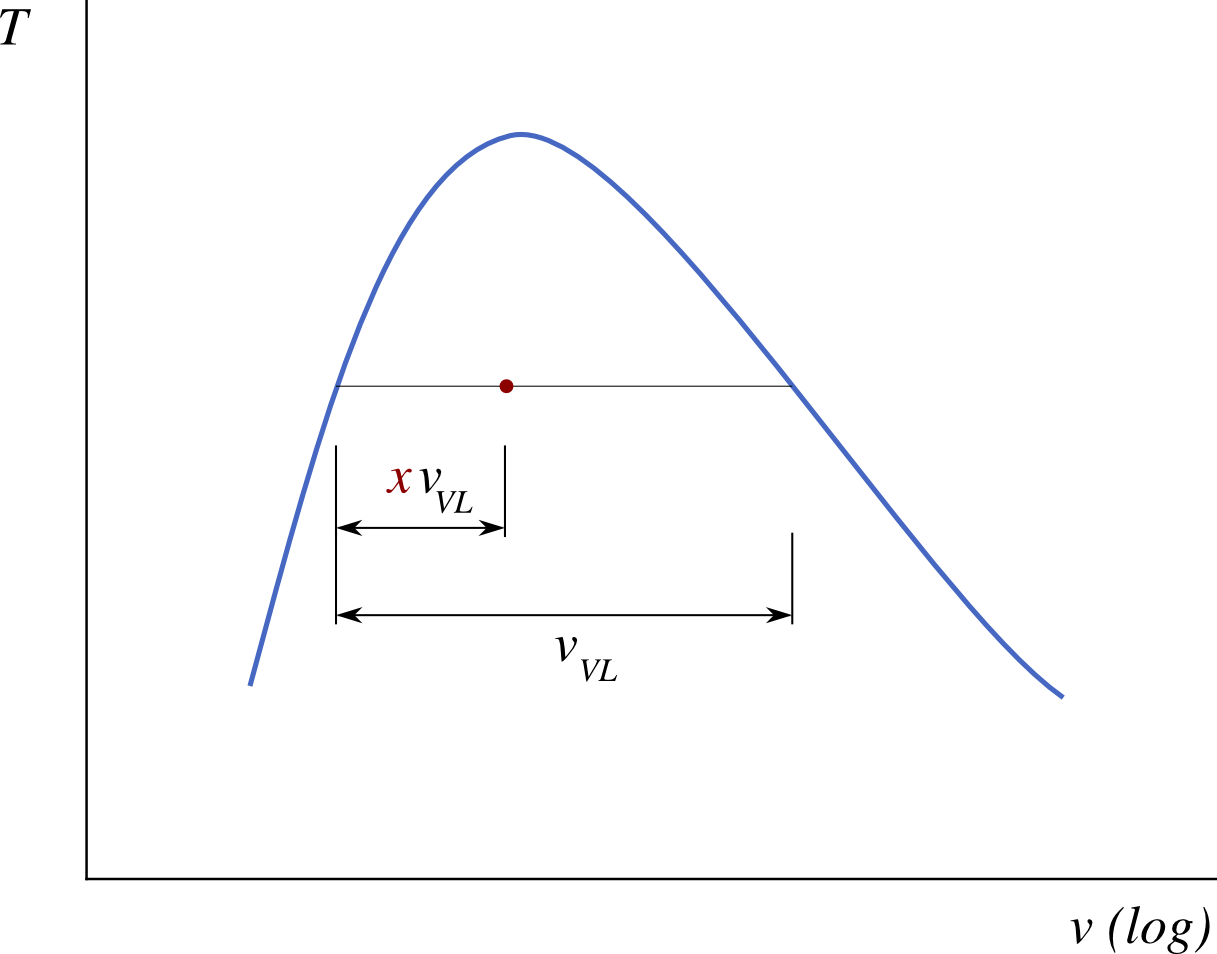
\includegraphics[width=\didacticpvdiagramwidth]{images/titre_tv_v1.png}
			\end{center}
			\supercaption{Le titre de la vapeur représenté par la position du point sur un diagramme $T-v$.}{\cczero \oc}
			\label{fig_notion_de_titre}
		\end{figure}
		
		Nous pouvons maintenant exprimer les propriétés $u$, $h$, et $v$ en fonction du titre :

		\begin{description}

			\item[L’enthalpie $h$]{d’un mélange liquide-vapeur est égale à la somme de l’enthalpie du liquide et de celle du gaz. On a ainsi, comme illustré en \cref{fig_titre_h} :
				\begin{IEEEeqnarray}{rCl}
					h_x 	& = & (1-x) h_L + x \ h_V 		\nonumber \\
						& = & h_L + x (h_V - h_L)				\nonumber \\
					h_x 	& = & h_L + x \ h_{LV}
					\label{eq_titre_enthalpie}
				\end{IEEEeqnarray}
				\begin{equationterms}
					\item où \tab $h_x$ 	\tab est l’enthalpie spécifique du mélange étudié (\si{\joule\per\kilogram}),
					\item 	\tab $x$ 	\tab son titre (sans unité),
					\item et \tab $h_{LV} \equiv h_V - h_L $ \tab (valeur tabulée) l’enthalpie spécifique de vaporisation à sa température (\si{\joule\per\kilogram}).
				\end{equationterms}

				\begin{figure}
					\begin{center}
						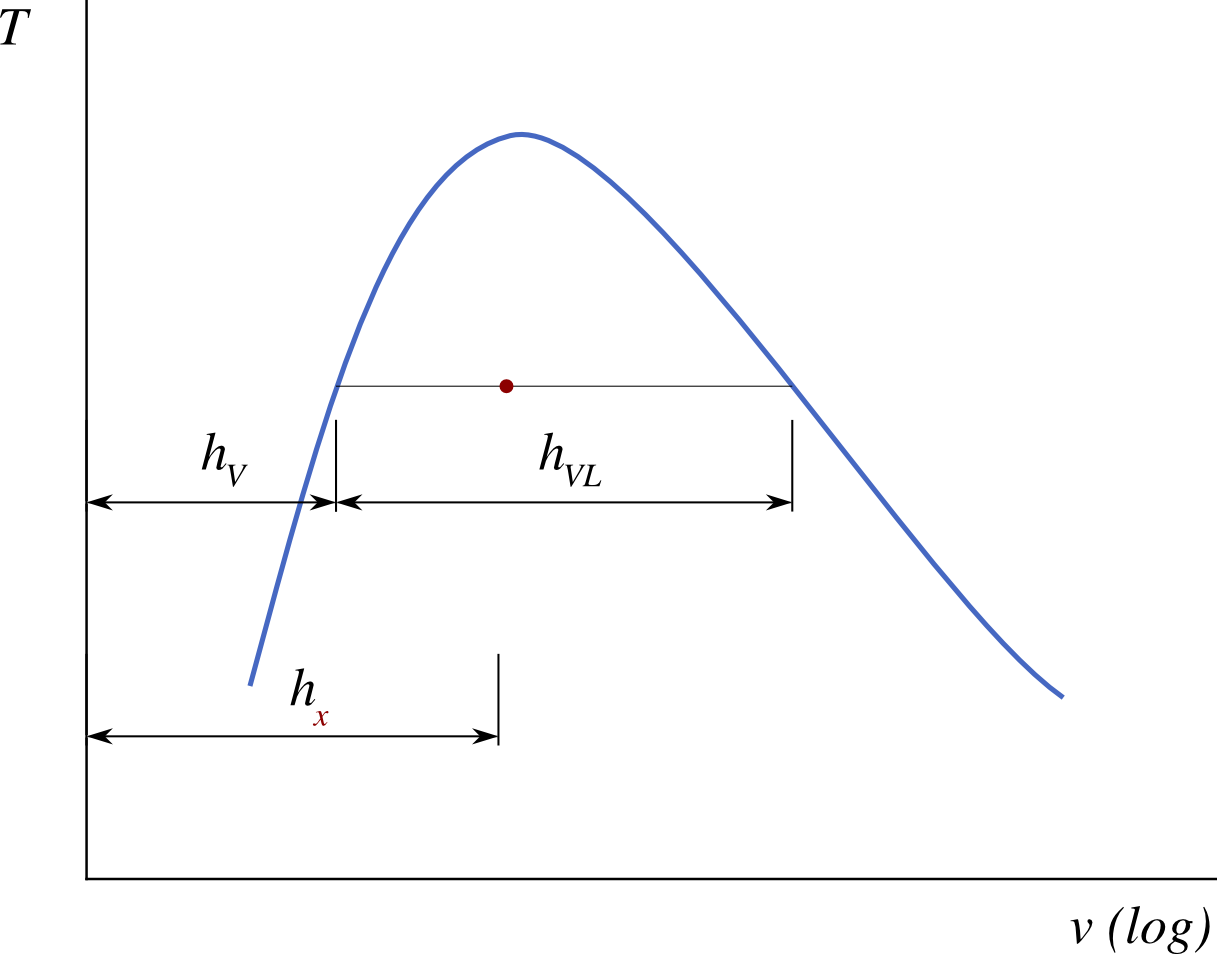
\includegraphics[width=\didacticpvdiagramwidth]{images/titre_tv_h.png}
					\end{center}
					\supercaption{Enthalpie $h_x$ d’un mélange en fonction des enthalpies à l’état saturé et de vaporisation.}{\cczero \oc}
					\label{fig_titre_h}
				\end{figure}
			} %end item

			\item[L’énergie interne $u$]{d’un mélange liquide vapeur se quantifie exactement de la même manière :
				\begin{equation}
					u_x = u_L + x \ u_{LV}
					\label{eq_titre_energie_interne}
				\end{equation}
				\begin{equationterms}
					\item où \tab $u_x$ 	\tab est l’énergie spécifique du mélange étudié (\si{\joule\per\kilogram}),
					\item 	\tab $x$ 	\tab son titre (sans unité),
					\item et \tab $u_{LV} \equiv u_V - u_L$ \tab (valeur tabulée) la différence des énergies internes spécifiques à saturation, à sa température (\si{\joule\per\kilogram}).
				\end{equationterms}
			} %end item

			\clearfloats %handmade
			\item[Le volume spécifique]{d’un mélange liquide-vapeur, enfin, se quantifie encore plus simplement. Le volume total du mélange est égal au volume du gaz plus celui du liquide, et donc :
				\begin{equation*}
					v_x = (1-x) v_L + x \ v_V
				\end{equation*}

				Toutefois, le volume spécifique $v_L$ du liquide saturé étant très petit devant celui de la vapeur%
					\footnote{Un court examen de l’abaque~n°2 révélera qu’il s’agit approximativement d’un facteur~\num{e3}. Il faut noter que ce facteur est très mal mis en évidence par les diagrammes $T-v$ et $p-v$ de ce chapitre, dont l’échelle des abscisses est logarithmique.}%
				, il peut être négligé et nous pouvons simplement écrire :
				\begin{equation}
					v_x \approx x \ v_V
					\label{eq_titre_volume_specifique}
				\end{equation}
				\begin{equationterms}
					\item où \tab $v_x$ 	\tab\tab est le volume spécifique du mélange étudié (\si{\metre\cubed\per\kilogram}),
					\item 	\tab $x$ 	\tab\tab son titre (sans unité),
					\item et \tab $v_V$ 	\tab (valeur tabulée) le volume spécifique de la vapeur saturée, à sa température (\si{\metre\cubed\per\kilogram}).
				\end{equationterms}

				Cette approximation est illustrée en \cref{fig_titre_v}.

				\begin{figure}
					\begin{center}
						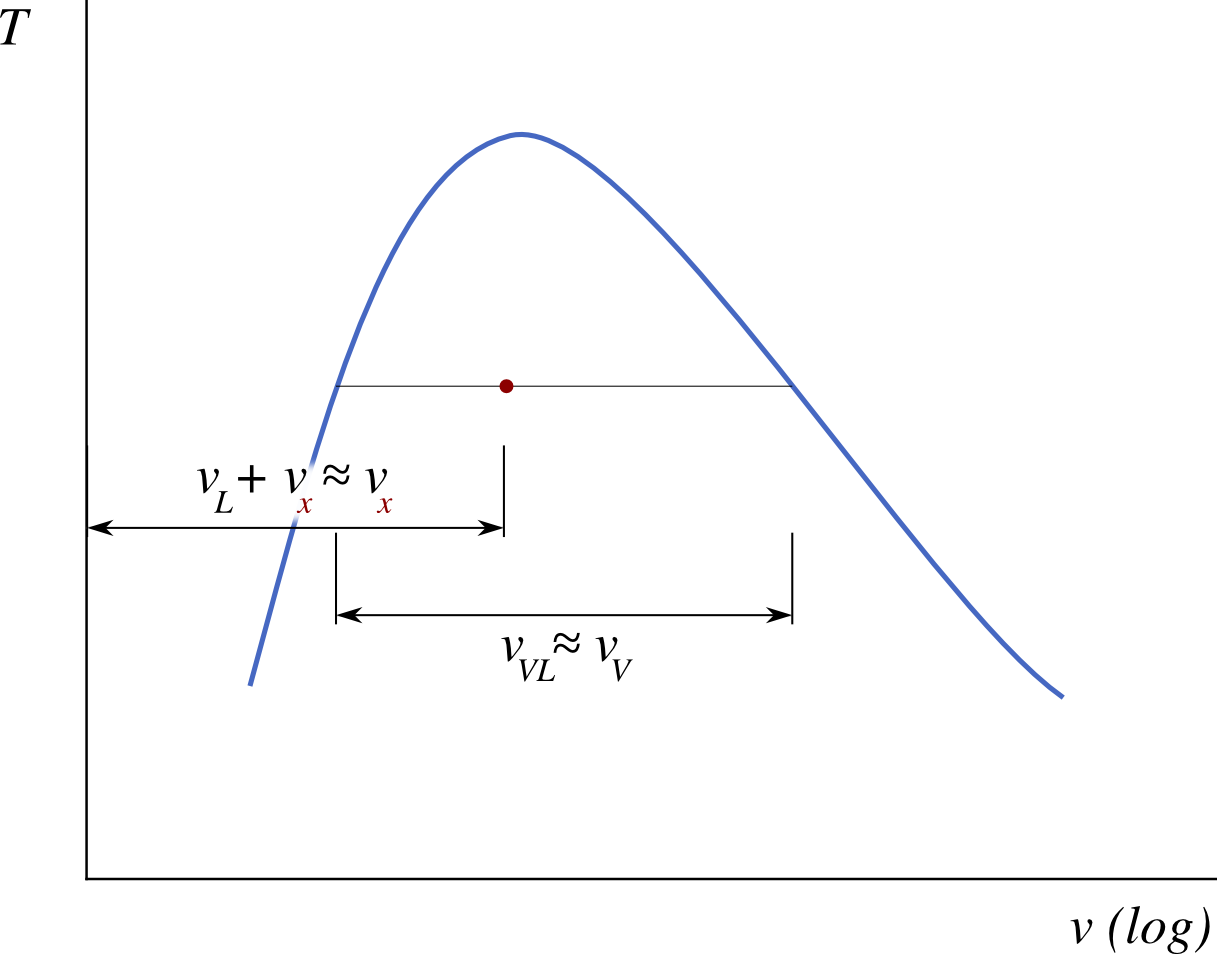
\includegraphics[width=\didacticpvdiagramwidth]{images/titre_tv_v2.png}
					\end{center}
					\supercaption{Approximations utilisées dans le calcul du volume occupé par un mélange liquide-vapeur.
				Il faut noter que l’échelle en abscisse est logarithmique : l’approximation n’est pas mise en valeur graphiquement.}{\cczero \oc}
					\label{fig_titre_v}
				\end{figure}
			} % end item

		\end{description}
		
		\clearfloats %handmade
		Nous pouvons maintenant utiliser les mêmes abaques~n°2 et~n°3 pour quantifier ce qui se passe entre les points de saturation.
		
			\begin{anexample}
			
			Quels sont l’énergie interne et le volume occupé par une masse de~\SI{3}{\kilogram} d’eau aux trois quarts vaporisée, à~\SI{115}{\degreeCelsius} ?
			
				\begin{answer}
				Nous avons un mélange liquide-vapeur et le titre est de~\num{0,75}. Nous allons à l’abaque~n°2 (extrait en \cref{abaque2extrait}) pour trouver la température de saturation \SI{115}{\degreeCelsius}.\\
				De là, on applique simplement l’\cref{eq_titre_energie_interne} : $u_x = u_L + \num{0,75}\times u_{LV} = \num{482,4} + \num{0,75}\times\num{2041} = \SI{2013,15}{\kilo\joule\per\kilogram}$.\\
				De même, avec l’\cref{eq_titre_volume_specifique} : $v_x = \num{0,75}\times v_{V} = \num{0,75}\times\num{1,0358} = \SI{0,77685}{\metre\cubed\per\kilogram}$.\\				
				On a donc $U = m \ u = \SI{8052,6}{\kilo\joule} $ et $V = m \ v = \SI{3,1074}{\metre\cubed}$.
				\end{answer}
			\end{anexample}
		
			\begin{anexample}
			
			Quel est le titre de l’eau à~\SI{2,5}{\bar} dont l’enthalpie est de~\SI{1500}{\kilo\joule\per\kilogram} ?
			
				\begin{answer}
				Nous avons un mélange liquide-vapeur ; on cherche dans l’abaque~n°3 (extrait en \cref{abaque3extrait}) la ligne correspondant à $p_\text{sat} = \SI{0,25}{\mega\pascal}$. Nous nous armons de l’\cref{eq_titre_enthalpie}.\\				
				De là, on obtient : $x = \frac{h_x - h_L}{h_{LV}} = \frac{\num{1500} - \num{535,3}}{\num{2181,1}} = \num{0,442} $.
				\begin{remark}Une courte vérification à la volée : à~\SI{1500}{\kilo\joule\per\kilogram} nous sommes bien au milieu environ du chemin entre $h_L \approx \num{500}$ et $h_V \approx \SI{2700}{\kilo\joule\per\kilogram}$. \end{remark}\end{answer}
			\end{anexample}





\section{Transformations élémentaires réversibles}
\label{ch_lv_evolutions_elementaires}

	Nous savons désormais quantifier les termes $pv$, $u$ et $h$ d’un liquide/vapeur dans tous les cas. Maintenant, nous nous proposons de faire comme au chapitre précédent (\S\ref{ch_gp_evolutions_elementaires}) : calculer les transferts d’énergie en jeu lorsqu’on comprime ou détend un liquide/vapeur selon des contraintes entièrement arbitraires de volume, pression ou température.


	\subsection{À quoi sert cette section de chapitre ?}
	\label{ch_lv_evolutions_elementaires_aquoisert}

		La réponse est la même qu’au \coursquatreshort (\S\ref{ch_gp_evolutions_elementaires_aquoisert}). Les évolutions de liquides/vapeurs que nous étudions ici sont très hypothétiques mais intéressantes pour deux raisons :

		\begin{enumerate}
			\item Le comportement d’un liquide/vapeur est intrinsèquement complexe. Ces évolutions élémentaires font figure de gymnastique et permettent d’apprendre à le décrire étape par étape ;
			\item Ces évolutions élémentaires sont des outils conceptuels que nous assemblerons plus tard, d’abord pour quantifier les limites théoriques des machines (au \coursseptshort), et enfin pour décrire le comportement des fluides à l’intérieur des machines réelles (au \coursneufshort).
		\end{enumerate}


	\subsection{Évolutions à pression constante}
	\label{ch_lv_isobare}

		\thermoquotebegin{O}
	On sait que lorsqu’on fait vaporiser de l’eau sous la pression atmosphérique, en vain lui ajoute-t-on continuellement de nouvelles quantités de chaleur au moyen du foyer, jamais la température de l’eau, non plus que celle de la vapeur, ne s’élèvent au-delà de 100° du thermomètre centigrade, ou 212° du thermomètre de Fahrenheit.
		\thermoquoteend{François-Marie Guyonneau de~Pambour, 1839}{\textit{Théorie de la machine à vapeur}~\cite{pambour1839}}

	Il est possible de chauffer ou refroidir un liquide/vapeur en maintenant sa pression constante (\cref{fig_lv_pression_constante}). Une évolution à pression constante est dite \vocab[évolutions!isobares]{isobare}\index{isobares, évolutions}.
		
		\begin{itemize}
			\item Dans un système fermé, on doit le contraindre avec une surface qui exerce une force constante quel que soit le volume ;
			\item Dans un système ouvert, il suffit de chauffer ou refroidir le gaz en le laissant s’écouler dans un conduit sans pièce mobile. C’est ce qui se passe dans une chaudière, par exemple.
		\end{itemize}

		\begin{figure}
			\begin{center}
				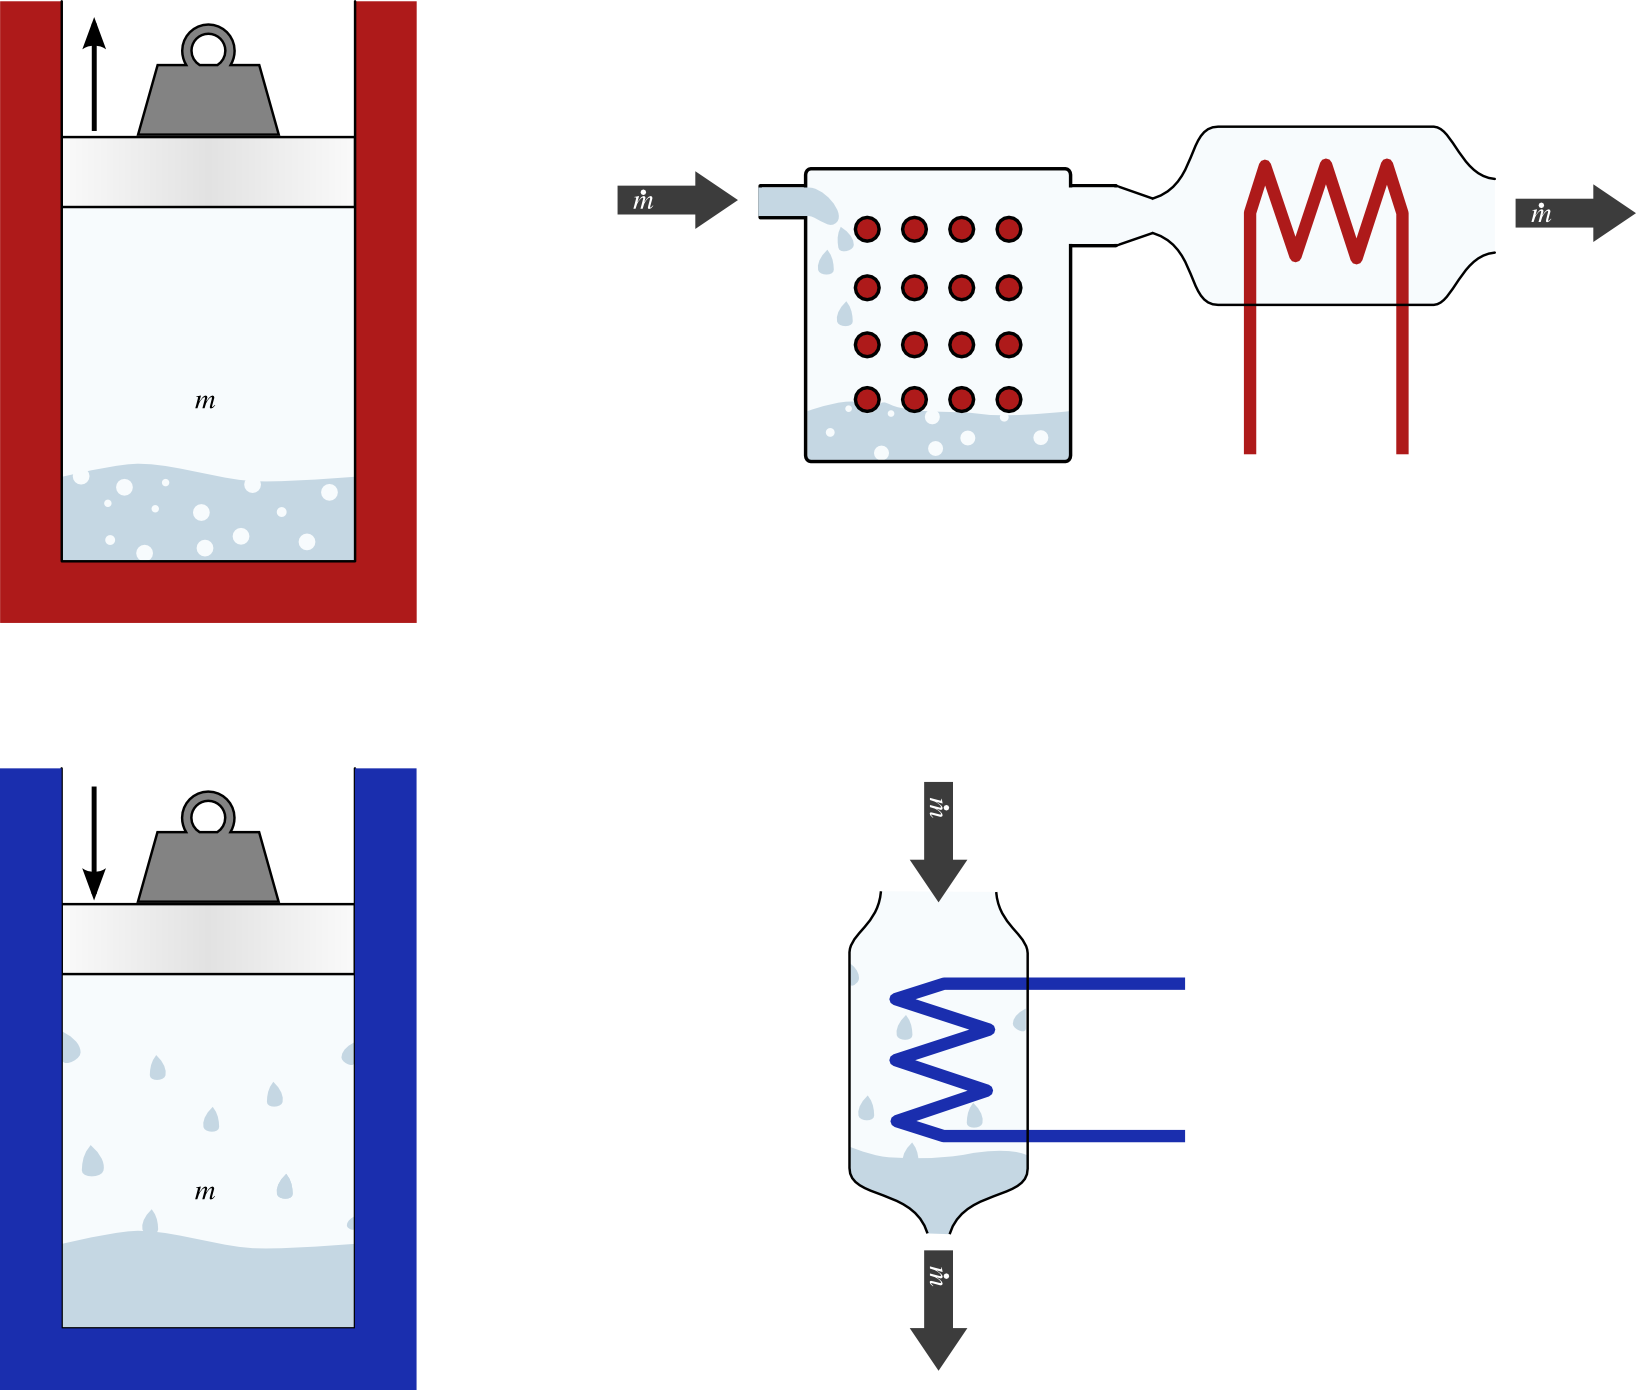
\includegraphics[width=11cm]{images/lv_isobare.png}
			\end{center}
			\supercaption{Évolution à pression constante (isobare) d’un liquide/vapeur. En système fermé (à gauche), le piston exerce une force constante tout au long de l’évolution. En système ouvert (à droite), aucun travail n’est effectué.}{\ccbysa \olivier}
			\label{fig_lv_pression_constante}
		\end{figure}
		
		\begin{figure}
			\begin{center}
				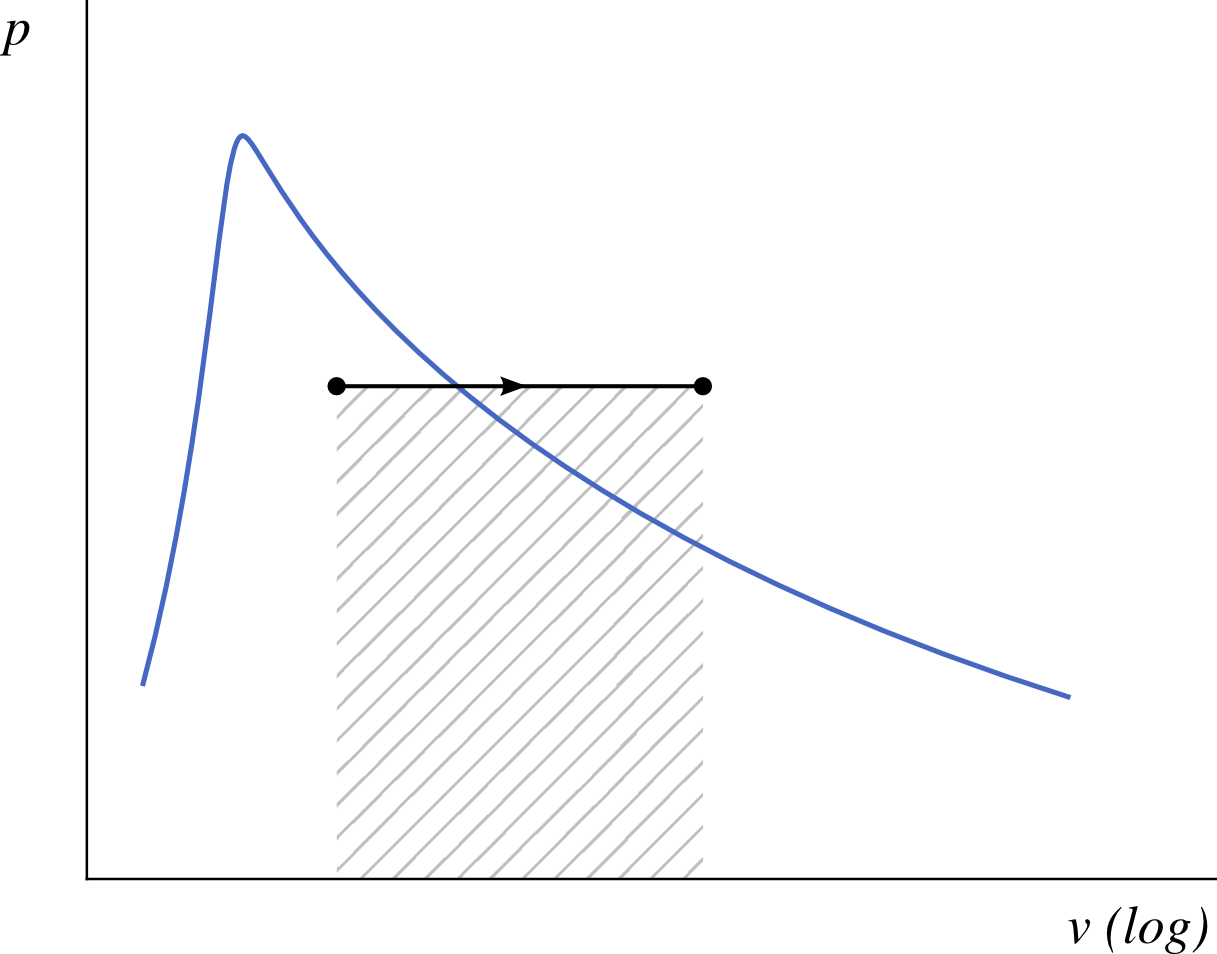
\includegraphics[width=\pvdiagramwidth]{images/pv_lv_isobare.png}
			\end{center}
			\supercaption{Réchauffement à pression constante d’un liquide/vapeur, représenté sur un diagramme pression-volume.}{\cczero \oc}
			\label{fig_lv_pression_constante_pv}
		\end{figure}	

		En système fermé, nous avons $q_{1\to2} + w_{1\to2} = \Delta u$ (\ref{eq_premier_principe_sf_min}). Si l’évolution est réversible, la chaleur et le travail peuvent être chacun quantifiés :
		\begin{IEEEeqnarray}{rCl}
			w_{1\to2} 	& = & - \int _1^2 p \diff v = -p_\text{cste} \int _1^2 \diff v	\nonumber \\
			w_{1 \to 2} 	& = & -p_\text{cste} \ \Delta v \label{eq_lv_sf_travail_isobare}
		\end{IEEEeqnarray}
		\begin{equationterms}
			\item lors d’une évolution réversible à pression constante $p_\text{cste}$, en système fermé.
		\end{equationterms}
		\begin{IEEEeqnarray}{rCl}
			q_{1\to2} 	& = & \Delta u - w_{1\to2} = \Delta u + p_\text{cste} \ \Delta v \nonumber \\
			q_{1 \to 2} 	& = & \Delta h \label{eq_lv_sf_chaleur_isobare}
		\end{IEEEeqnarray}
		\begin{equationterms}
			\item lors d’une évolution réversible à pression constante, en système fermé.
		\end{equationterms}

		Lorsque l’évolution se fait en système ouvert, nous avons $q_{1\to2} + w_{1\to2} = \Delta h$ (\ref{eq_petite_sfee_deltas_h}). Si l’évolution est réversible, la chaleur et le travail peuvent être chacun quantifiés :
		\begin{IEEEeqnarray}{rCl}
			w_{1\to2} 	& = & \int _1^2 v \diff p \nonumber \\
			w_{1\to2} 	& = & 0
			\label{eq_lv_travail_isobare}
		\end{IEEEeqnarray}
		\begin{equationterms}
			\item lors d’une évolution réversible à pression constante, en système ouvert.
		\end{equationterms}
		\begin{IEEEeqnarray}{rCl}
			q_{1\to2} 	& = & \Delta h - w_{1\to2} \nonumber \\
			q_{1 \to 2} 	& = & \Delta h
			\label{eq_lv_chaleur_isobare}
		\end{IEEEeqnarray}
		\begin{equationterms}
			\item lors d’une évolution réversible à pression constante, en système ouvert.
		\end{equationterms}


		\begin{anexample}
			Combien de travail et de chaleur faut-il pour chauffer lentement \SI{2}{\kilogram} d’eau liquide saturée à pression constante (\SI{3}{\bar}), jusqu’à ce que le volume atteigne~\SI{1}{\metre\cubed} ?
			
				\begin{answer}
				Nous partons de l’état liquide saturé, à $v_1 = v_L$ et $h_1 = h_L$.
				Nous avons besoin du volume spécifique et de l’enthalpie finaux pour pouvoir quantifier $W_{1\to2}$ et $Q_{1\to2}$. Le volume final sera $v_2 = \frac{V_2}{m} = \SI{0,5}{\metre\cubed\per\kilogram}$.
					\begin{remark}On remarque que $v_2$ est inférieur à $v_V$ à notre température. À la fin du réchauffement, l’eau sera toujours partiellement liquide et nous allons devoir calculer son titre.\end{remark}
					\begin{remark}Mélange liquide-vapeur ? On se dirige vers les abaques~n°2 et~n°3. Nous connaissons la pression (\SI{0,3}{\mega\pascal}), c’est donc l’abaque~n°3 qu’il nous faut.\end{remark}
				
				Le titre final est $x_2 \approx \frac{v_x}{v_{V}} = \frac{\num{0,5}}{\num{0,60576}} = \num{0,825} $ (\ref{eq_titre_volume_specifique}). On a donc $h_2 = h_L + x_2 \ h_{LV} = \num{561,4} + \num{0,825}\times\num{2163,5} = \SI{2347,2}{\kilo\joule\per\kilogram}$ (\ref{eq_titre_enthalpie}).
				
				On obtient le travail avec l’\cref{eq_lv_travail_isobare} : $W_{1\to2} = m \ w_{1\to2} = - m \ p_\text{cste} \ \Delta v = - 2 \times \num{0,3e6} \times(\num{0,5} - \num{0,001073}) = \SI{-2,994e5}{\joule} = \SI{-299,4}{\kilo\joule} $.
				
				Enfin, la chaleur avec l’\cref{eq_lv_chaleur_isobare} : $Q_{1\to2} = m \ q_{1\to2} = m \ \Delta h = 2 \times (\num{2347,2e3} - \num{561,4e3}) = \SI{+3,5715e6}{\joule} = \SI{+3571,5}{\kilo\joule}$.
				
				
				\begin{remark}Le transfert de chaleur mis en jeu est dix fois plus important que le travail. Ici, nous chauffons beaucoup et le fluide, à basse pression, travaille peu.\end{remark}
				\begin{remark}Il est probablement plus simple et moins risqué de retrouver ces équations~\ref{eq_lv_travail_isobare} et~\ref{eq_lv_chaleur_isobare} à la main que de tenter de les mémoriser.\end{remark}\end{answer}
			\end{anexample}


		On peut remarquer que lorsqu’on chauffe l’eau en mélange liquide/vapeur (sous la courbe de saturation), l’augmentation de volume est formidable. Concrètement, il suffit de quelques millilitres d’eau liquide pour obtenir une expansion de plusieurs litres à pression constante, avec une température très modérée et constante. C’est la raison pour laquelle tous les premiers moteurs, au \textsc{xix}\ieme siècle, ont fonctionné à l’eau plutôt qu’avec de l’air. La grande démultiplication du volume permettait des moteurs plus compacts et avec de grands débattements (mécanismes plus simples), la pression constante évitait les à-coups, et les faibles températures permettaient l’usage de matériaux simples : une combinaison de facteurs avantageuse avec une technologie peu avancée.
		
		Nous verrons aux \courssept et \coursneuf que ces avantages se traduisent hélas par une inefficacité
pharaonique. Pour s’en affranchir, il faudra monter en température : ce sera pour le \textsc{xx}\ieme siècle.


	\subsection{Évolutions à volume constant}
	\label{ch_lv_isochores}

		Il est possible de chauffer ou refroidir un liquide/vapeur en maintenant son volume constant (\cref{fig_lv_isochore}). Une évolution à volume constant est dite \vocab[évolutions!isochores]{isochore}\index{isochores, évolutions}.

		\begin{figure}
			\begin{center}
				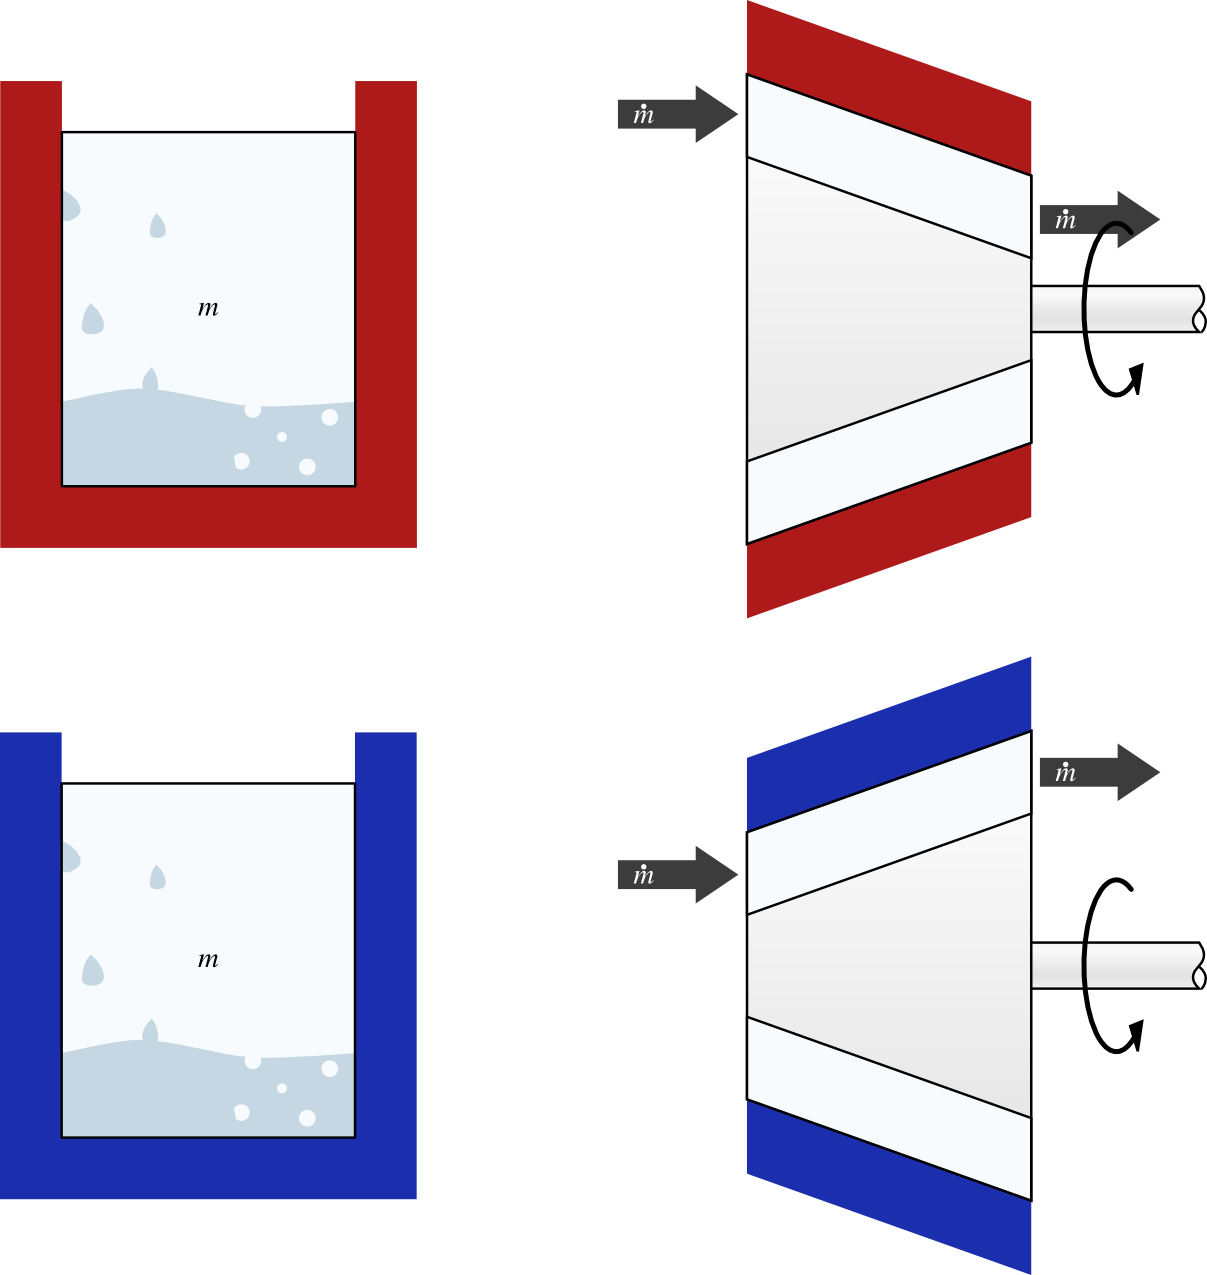
\includegraphics[width=8cm]{images/lv_isochore.png}
			\end{center}
			\supercaption{Évolution à volume constant (isochore) d’un liquide/vapeur. En système fermé (à gauche), le volume est bloqué et aucun travail n’est effectué. En système ouvert (à droite), on doit comprimer le fluide pendant qu’on le chauffe et le détendre pendant qu’on le refroidit, pour pouvoir maintenir le volume spécifique constant.}{\ccbysa \olivier}
			\label{fig_lv_isochore}
		\end{figure}
		
		\begin{figure}
			\begin{center}
				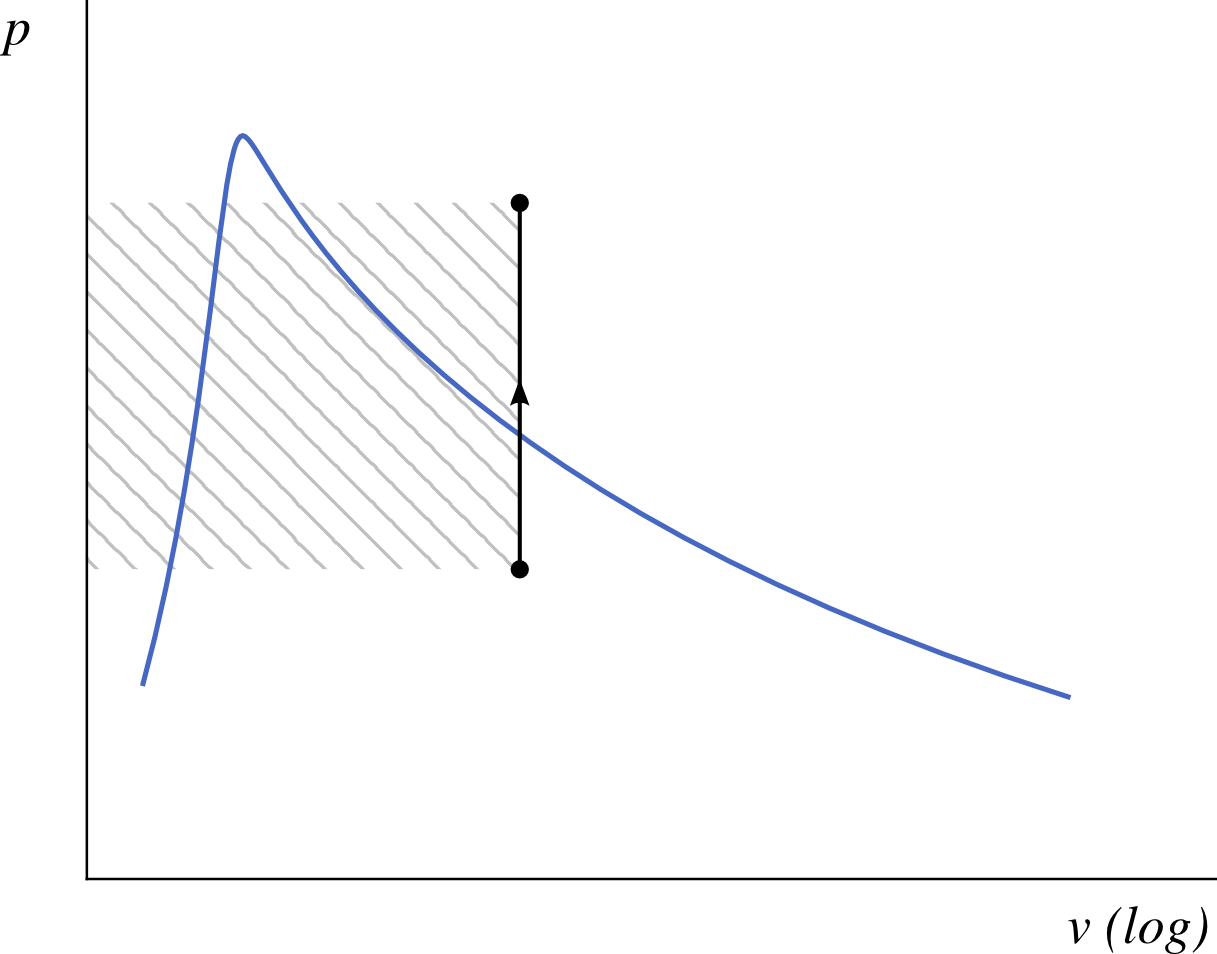
\includegraphics[width=\pvdiagramwidth]{images/pv_lv_isochore.png}
			\end{center}
			\supercaption{Réchauffement à volume constant d’un liquide/vapeur, représenté sur un diagramme pression-volume.}{\cczero \oc}
			\label{fig_pv_lv_isochore}
		\end{figure}	

		\begin{itemize}
			\item Dans un système fermé, on peut chauffer ou refroidir le liquide/vapeur dans un réservoir fixe et fermé ;
			\item Dans un système ouvert, la situation est plus complexe. On doit compresser le liquide/vapeur pendant qu’on le réchauffe pour éviter que son volume n’augmente ; de même, pour éviter que son volume ne baisse en le refroidissant, il faut le détendre.
		\end{itemize}	
		
		En système fermé, nous avons $q_{1\to2} + w_{1\to2} = \Delta u$. La chaleur et le travail peuvent être chacun quantifiés :
		\begin{IEEEeqnarray}{rCl}
			w_{1\to2} 	& = & - \int _1^2 p \diff v	\nonumber \\
			w_{1\to2} 	& = & 0 \label{eq_lv_sf_travail_isochore}
		\end{IEEEeqnarray}
		\begin{equationterms}
			\item lors d’une évolution à volume constant, en système fermé.
		\end{equationterms}
		\begin{IEEEeqnarray}{rCl}
			q_{1\to2} 	& = & \Delta u - w_{1\to2} \nonumber \\
			q_{1\to2} 	& = & \Delta u \label{eq_lv_sf_chaleur_isochore}
		\end{IEEEeqnarray}
		\begin{equationterms}
			\item lors d’une évolution à volume constant, en système fermé.
		\end{equationterms}

		
		Lorsque l’évolution se fait en système ouvert, nous avons $q_{1\to2} + w_{1\to2} = \Delta h$. Si l’évolution est réversible, la chaleur et le travail peuvent être chacun quantifés :
		\begin{IEEEeqnarray}{rCl}
			w_{1\to2} 	& = & \int _1^2 v \diff p = v_\text{cste} \int_1^2 \diff p \nonumber \\
			w_{1\to2} 	& = & v_\text{cste} \ \Delta p \label{eq_lv_so_travail_isochore}
		\end{IEEEeqnarray}
		\begin{equationterms}
			\item lors d’une évolution réversible à volume constant, en système ouvert.
		\end{equationterms}
		\begin{IEEEeqnarray}{rCl}
			q_{1\to2} 	& = & \Delta h - w_{1\to2} = \Delta h - v_\text{cste} \ \Delta p \nonumber \\
			q_{1\to2} 	& = & \Delta u \label{eq_lv_so_chaleur_isochore}
		\end{IEEEeqnarray}
		\begin{equationterms}
			\item lors d’une évolution réversible à volume constant, en système ouvert.
		\end{equationterms}

		Remarquons qu’en fonction de son titre au départ, un mélange liquide-vapeur peut devenir entièrement liquide ou bien entièrement gazeux, lorsqu’il est chauffé à volume constant.



	\subsection{Évolutions à température constante}
	\label{ch_lv_isothermes}


		Il est possible de chauffer ou refroidir un liquide/vapeur en maintenant sa température constante (\cref{fig_lv_isotherme}). Une évolution à température constante est dite \vocab[évolutions!isothermes]{isotherme}\index{isothermes, évolutions}.

		\begin{figure}
			\begin{center}
				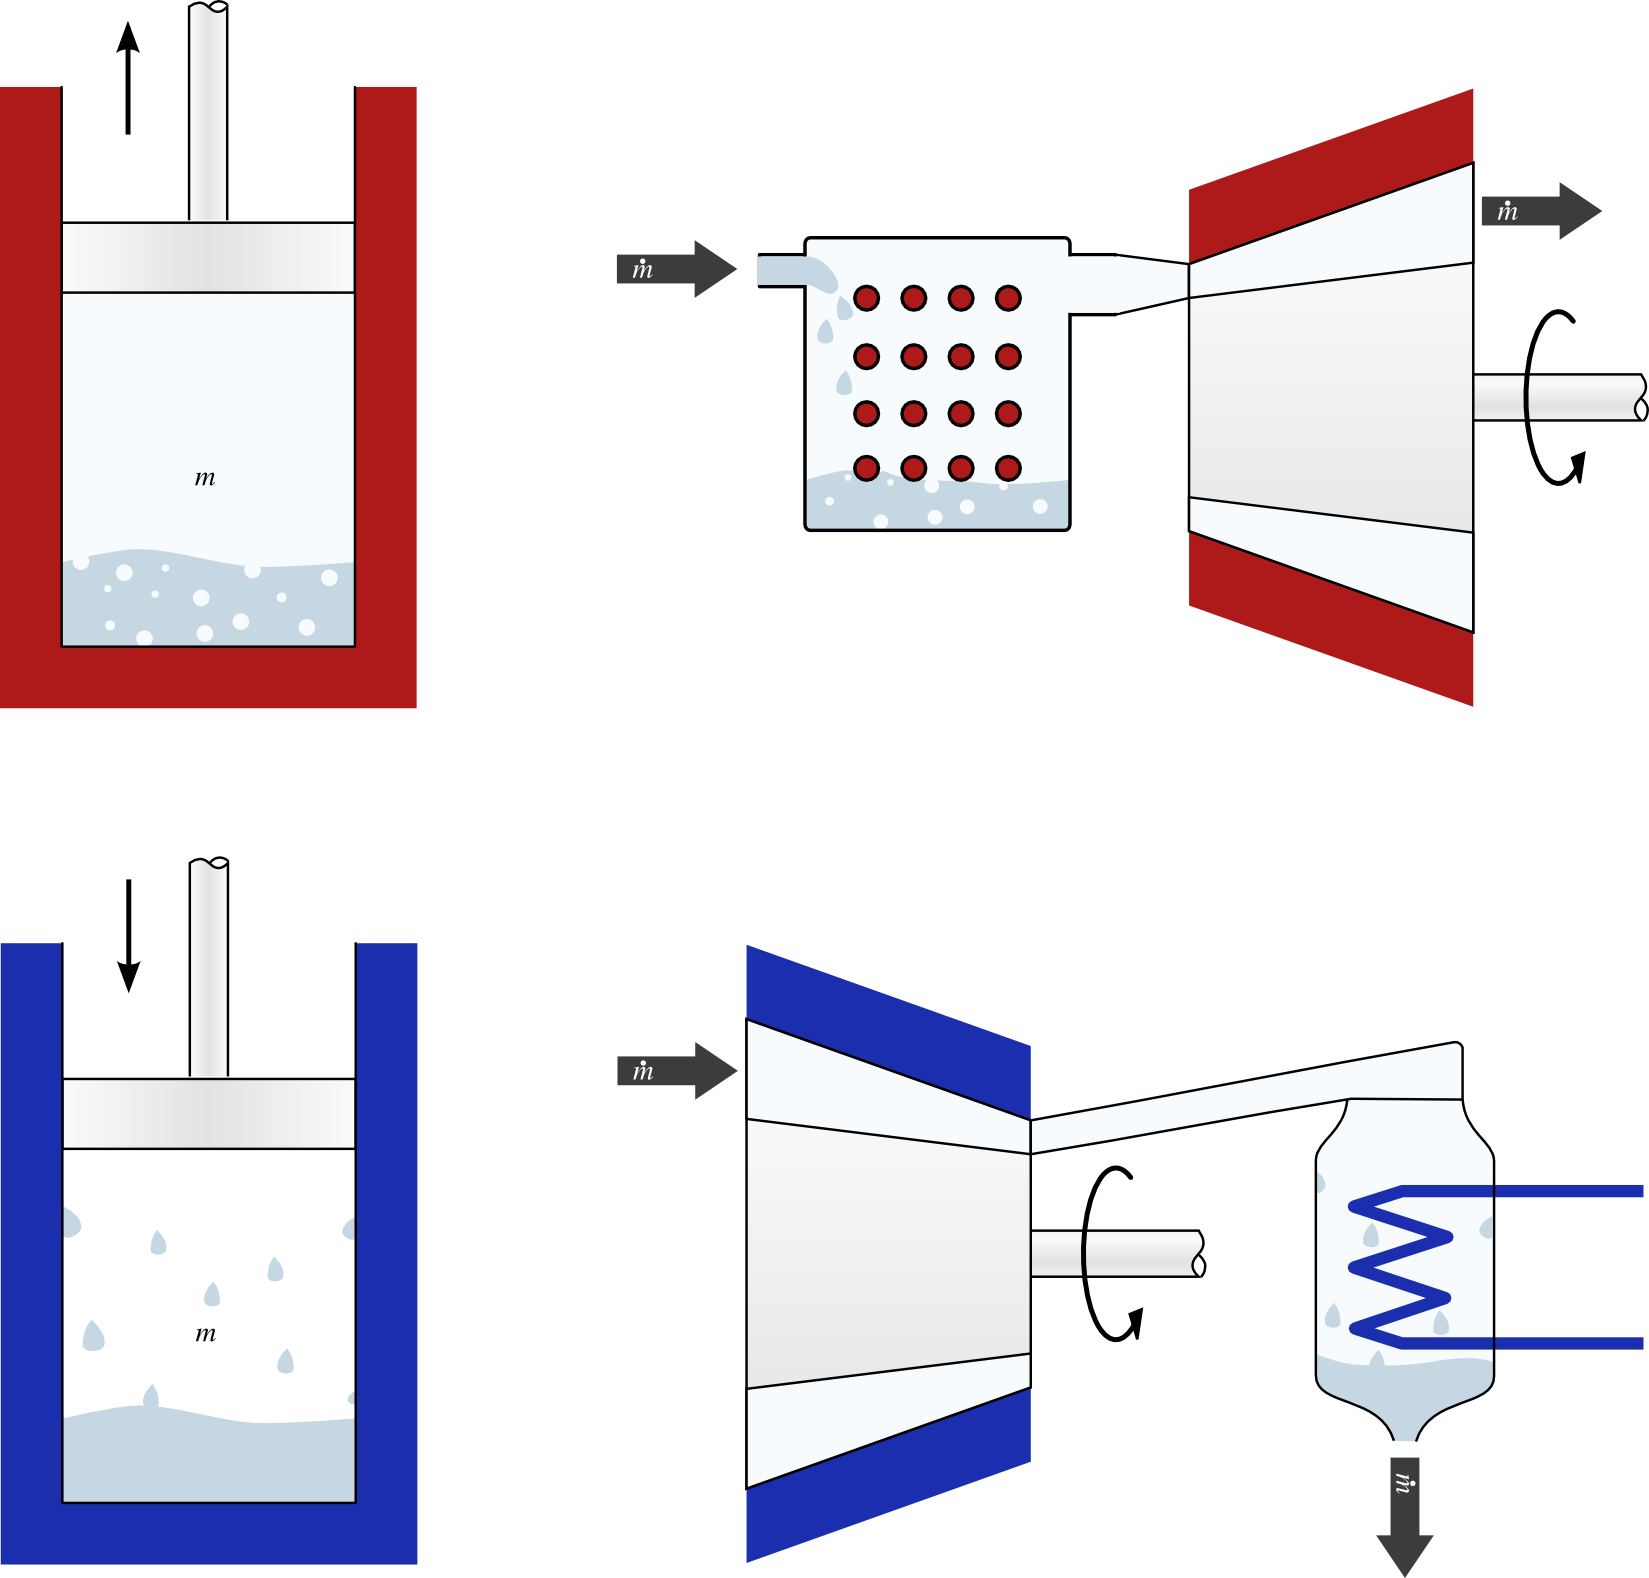
\includegraphics[width=11cm]{images/lv_isotherme.png}
			\end{center}
			\supercaption{Évolution à température constante (isotherme) d’un liquide/vapeur. En système fermé (à gauche), on laisse travailler le gaz sur un piston pendant qu’on le chauffe, et à l’inverse, on lui fournit du travail lorsqu’on le refroidit. En système ouvert (à droite), les mêmes manipulations sont effectuées en flux continu.}{\ccbysa \olivier}
			\label{fig_lv_isotherme}
		\end{figure}
		
		\begin{figure}
			\begin{center}
				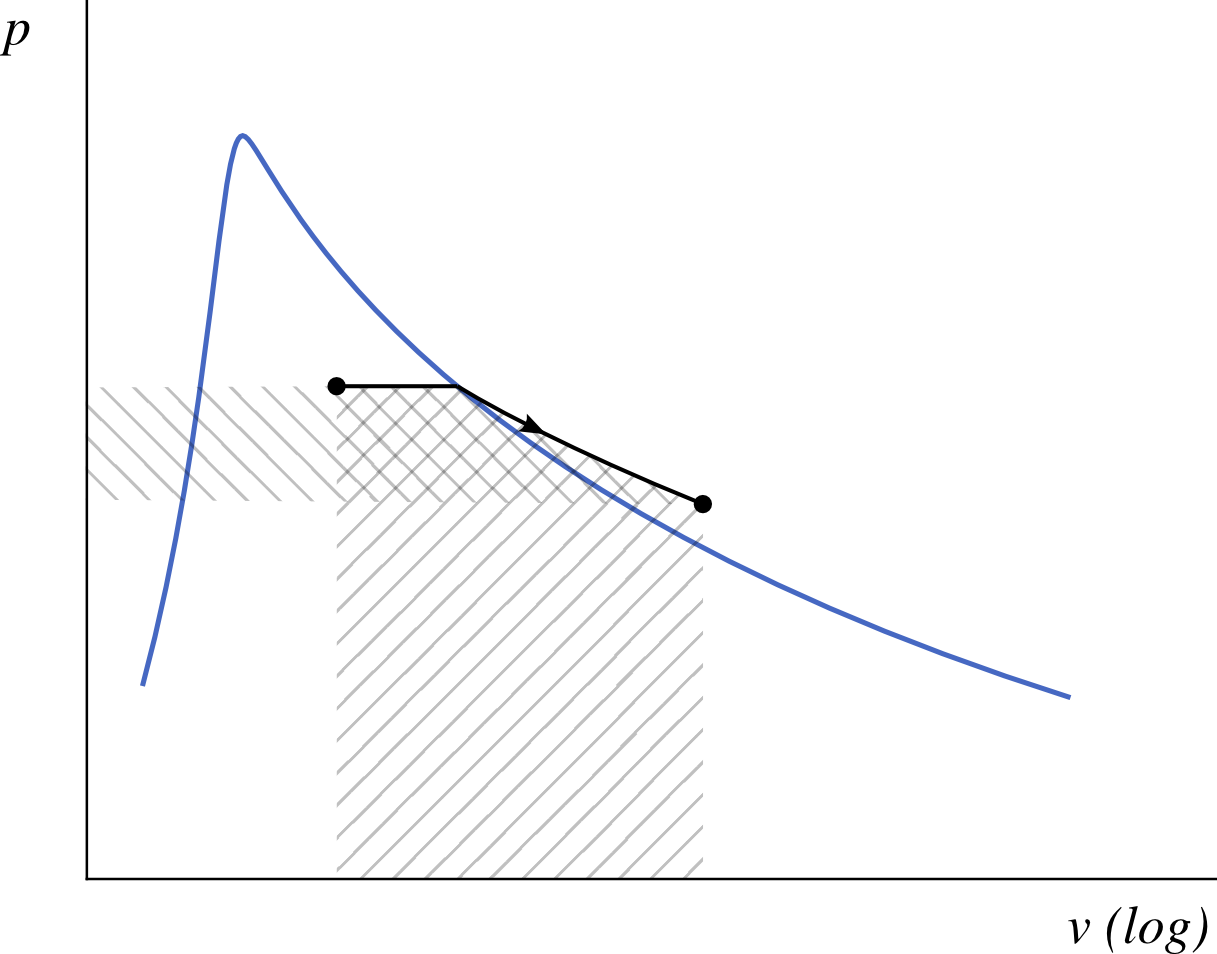
\includegraphics[width=\pvdiagramwidth]{images/pv_lv_isotherme.png}
			\end{center}
			\supercaption{Détente (réchauffement) à température constante d’un liquide/vapeur, représenté sur un diagramme pression-volume.}{\cczero \oc}
			\label{fig_pv_lv_isotherme}
		\end{figure}

		Lorsque le fluide est en mélange de phases (au centre de la courbe de saturation), l’évolution à température constante se fait aussi à pression constante, comme décrit en section~\S\ref{ch_lv_isobare} plus haut. Pour quantifier les transferts d’énergie, nous n’avons qu’à nous référer aux équations~\ref{eq_lv_travail_isobare} et~\ref{eq_lv_chaleur_isobare}.

		Par contre, dès que l’on franchit la courbe de saturation, rien ne va plus. Lorsque la saturation est atteinte, la pression se met à décroître et nous n’avons pas de moyen analytique de décrire cette évolution.
		
		La conséquence est que pour l’instant, nous ne pouvons pas quantifier le travail et la chaleur mis en jeu lorsque l’on fait évoluer de la vapeur à température constante !

		Lorsque nous aurons introduit le concept de l’\vocab{entropie} dans le \courshuitshort, nous disposerons d’un moyen simple de quantifier le flux de chaleur dans une évolution à température constante.
		
			\begin{anexample}
			
			Combien de travail et de chaleur faut-il pour chauffer lentement \SI{2}{\kilogram} d’eau liquide saturée à température constante (\SI{130}{\degreeCelsius}), jusqu’à ce que son volume atteigne \SI{1}{\metre\cubed} ?
			
				\begin{answer}
				On observe d’abord l’état final. Le volume final sera $v_2 = \frac{V_2}{m} = \SI{0,5}{\metre\cubed\per\kilogram} $, ce qui est inférieur à $v_V$ à notre température. Conclusion : même à la fin du réchauffement, l’eau sera toujours partiellement liquide.
				
				L’évolution se fera donc aussi à pression constante (à la pression de saturation, $p_{\text{sat.} \SI{130}{\degreeCelsius}} = \SI{0,27028}{\mega\pascal} $). Le calcul est exactement le même que pour l’exemple développé en \S\ref{ch_lv_isobare}. On obtient un titre de~\num{0,749}, une quantité de travail $W_{1\to2} = \SI{-269,7}{\kilo\joule}$ et de chaleur $Q_{1\to2} = \SI{+3256,2}{\kilo\joule}$.				
				
				\begin{remark}Tant que l’on est en mélange liquide/vapeur (sous la courbe de saturation), température constante = pression constante. Aucun problème.\end{remark}\end{answer}
			\end{anexample}
			
			
			\begin{anexample}
			
			On reprend la même question avec un volume final plus grand : \SI{2}{\metre\cubed}. Combien faut-il de chaleur et de travail ?
					
				\begin{answer}
				On ne peut pas encore répondre simplement à cette question ! Le volume spécifique final dépasse $v_V$ et la pression chute donc sur la fin de l’évolution (\cref{fig_pv_lv_isotherme}).
				
				Pour répondre, il nous faudrait un moyen de prédire la pression à la fin de l’évolution. Sinon, nous sommes condamnés à interpoler entre les lignes \emph{et les colonnes} de l’abaque~n°1 (en cherchant un volume $v_2$ à~\SI{130}{\degreeCelsius}), ce qui serait imprécis et malcommode.
				
				\begin{remark}Avec le modèle du gaz parfait, nous pouvions écrire que $p v = \text{cste}$ à température constante, et donc prédire toutes les propriétés à la fin de la détente. Mais avec un liquide/vapeur, cela ne fonctionne plus.\end{remark}
				\begin{remark}Après le \courshuitshort et comme pour l’exemple précédent, nous saurons utiliser le génial concept de l’\vocab{entropie} pour répondre à cette question.\end{remark}\end{answer}
			\end{anexample}




	\subsection{Évolutions adiabatiques réversibles}
		\label{ch_lv_isentropiques}

		Une évolution \vocab[évolutions!adiabatiques]{adiabatique}\index{adiabatiques, évolutions} est une évolution au cours de laquelle il n’y a aucun transfert de chaleur (\cref{fig_lv_isentropique}). On peut obtenir cela en recouvrant le récipient ou le conduit avec une épaisse couche d’isolant thermique.
		
		\thermoquotebegin{O}
		On me permettra peut-être ici de me référer à un fait prouvé par Rankine et moi-même : lorsqu’une quantité de vapeur, à sa masse volumique maximale et incluse par une surface impénétrable à la chaleur, se détend et par cette manière déplace une partie mobile de cette surface cloisonnante, par exemple un piston, avec sa pleine force d’expansion, une partie de la vapeur doit se condenser~\jecourte.
		\thermoquoteend{Rudolf Clausius, 1856}{\textit{Über die Anwendung der mechanischen Wärmetheorie auf~die Dampfmaschine}~\cite{clausius1856}\onlyamphibook{\vspace{8em}}} %handmade vspace
		
		Comme pour un gaz parfait, la température est nécessairement amenée à varier dans une telle évolution, puisque le travail est non-nul. Nous notons aussi que les courbes des évolutions adiabatiques réversibles tracées sur un diagramme pression-volume croisent toujours la courbe de saturation. Autrement dit, une vapeur sèche détendue lentement sans transfert de chaleur sera, tôt ou tard, amenée à se condenser. C’est un fait qui aura des conséquences importantes au \coursneuf.

		Une évolution adiabatique \emph{réversible}\index{évolutions!adiabatiques réversibles}\index{adiabatiques réversibles, évolutions} est effectuée infiniment lentement. Un piston dans un cylindre devra pour cela être déplacé infiniment lentement, et une turbine en flux continu devra pour cela être infiniment longue. Les évolutions adiabatiques servent de référence, d’objectif théorique, pour quantifier les performances des turbines réelles, que nous étudierons au \coursneufshort.

		\begin{figure}
			\begin{center}
				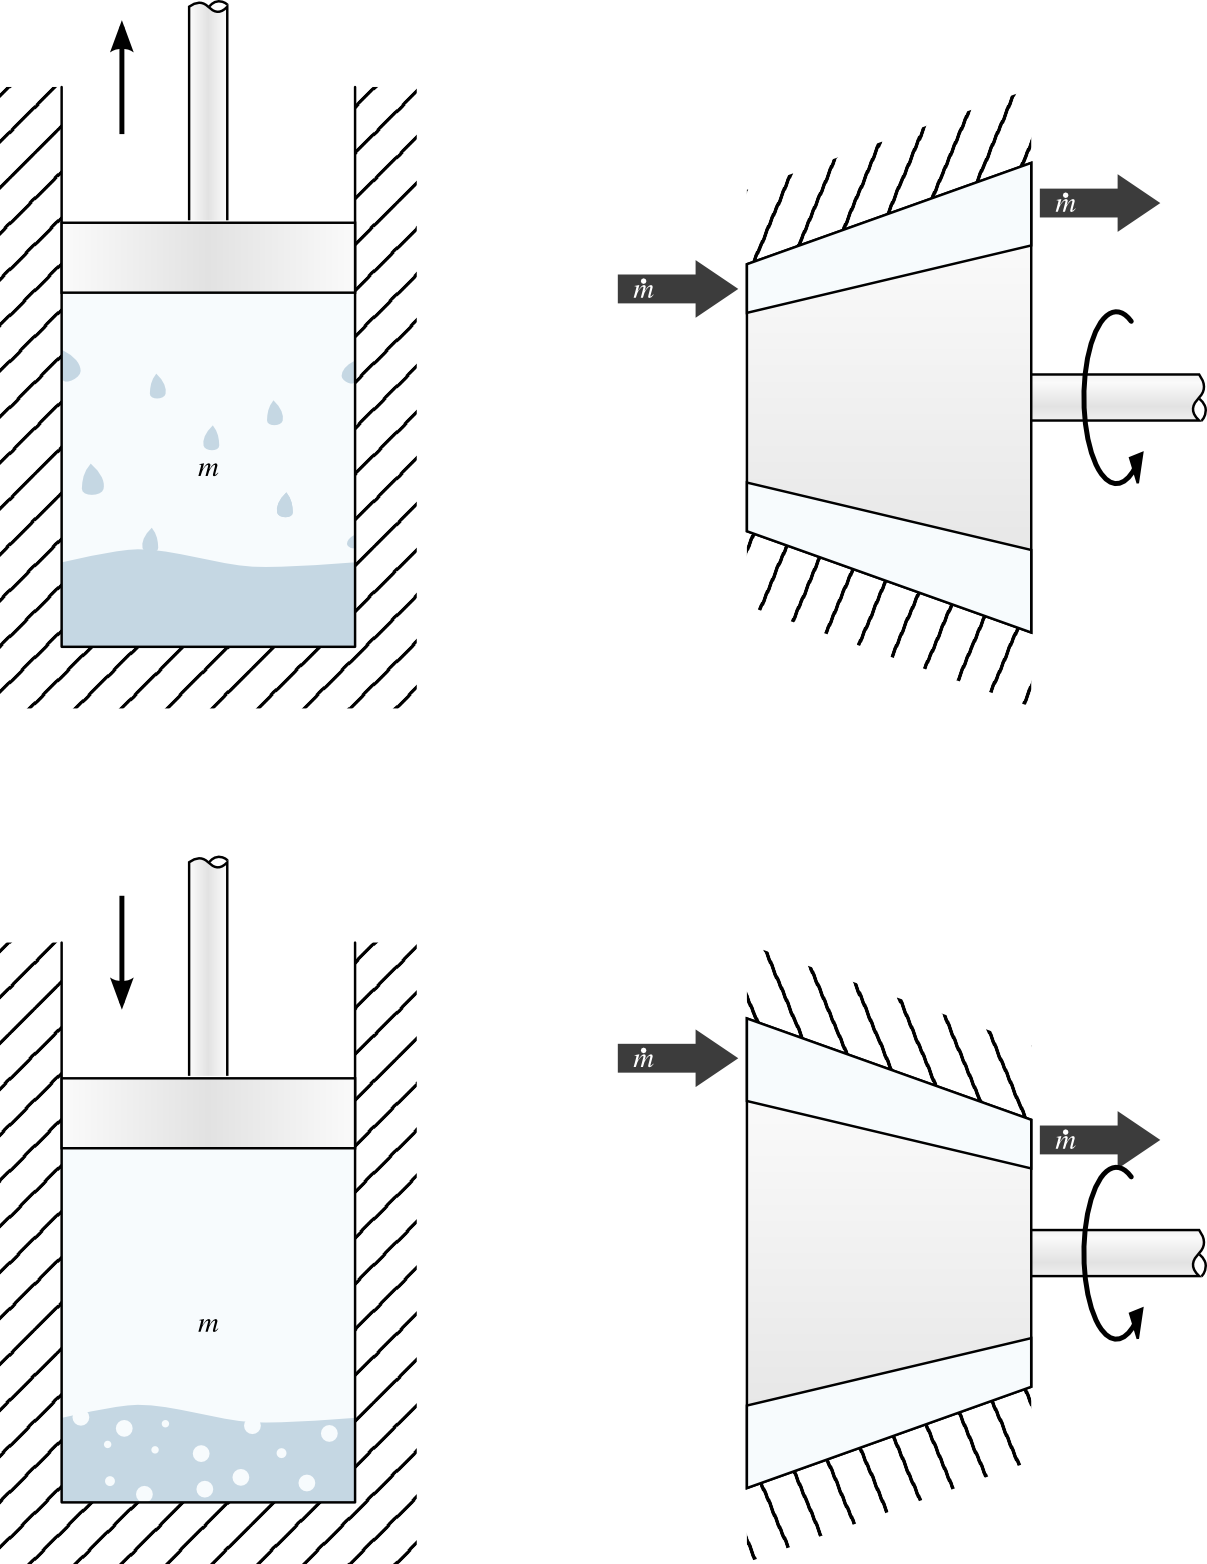
\includegraphics[width=8cm]{images/lv_isentropique.png}
			\end{center}
			\supercaption{Évolution adiabatique réversible (isentropique) d’un liquide/vapeur. En système fermé (à gauche) comme en système ouvert (à droite), le fluide est parfaitement isolé, de sorte qu’il n’y ait aucun transfert de chaleur, même si sa température varie.}{\ccbysa \olivier}
			\label{fig_lv_isentropique}
		\end{figure}
		
		\begin{figure}
			\begin{center}
				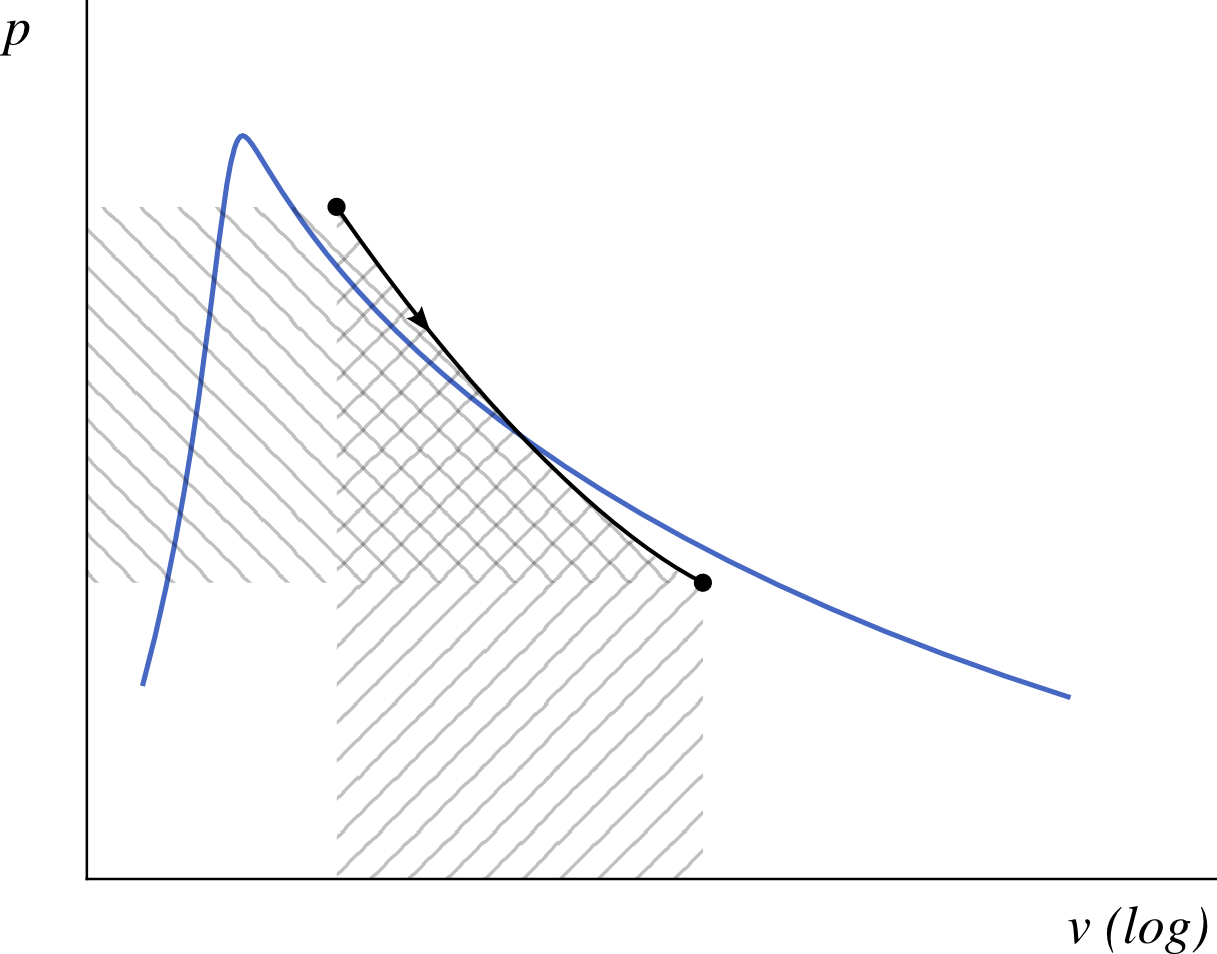
\includegraphics[width=\pvdiagramwidth]{images/pv_lv_isentropique.png}
			\end{center}
			\supercaption{Détente adiabatique réversible d’un liquide/vapeur, représentée sur un diagramme pression-volume.}{\cczero \oc}
			\label{fig_pv_lv_isentropique}
		\end{figure}

		
		Dans n’importe quelle évolution adiabatique, le transfert de chaleur est nul :
		\begin{equation}
			q_{1\to2} = 0
			\label{eq_lv_travail_adiabatique}
		\end{equation}
		\begin{equationterms}
			\item pour toute évolution adiabatique.
		\end{equationterms}

		Le travail s’exprime donc simplement :
		\begin{equation}
			w_{1\to2} = \Delta u
			\label{eq_lv_travail_adiabatique_sf}
		\end{equation}
		\begin{equationterms}
			\item pour toute évolution adiabatique en système fermé ;
		\end{equationterms}
		\begin{equation}
			w_{1\to2} = \Delta h
			\label{eq_lv_travail_adiabatique_so}
		\end{equation}
		\begin{equationterms}
			\item pour toute évolution adiabatique en système ouvert.
		\end{equationterms}


		Comment quantifier ce $\Delta u$ ou ce $\Delta h$ ? Prenons l’exemple d’une détente adiabatique, en partant de~\SI{40}{\bar} et~\SI{500}{\degreeCelsius}. On tente d’extraire le maximum de travail de la vapeur avant de la rejeter à pression atmosphérique (\SI{1}{\bar}).
		
		\begin{itemize}
			\item Si la détente est complètement irréversible (très brutale), alors le travail est de zéro. La vapeur est rejetée avec la même quantité d’énergie ($u$, $h$) qu’à l’entrée.
			\item Plus on effectue la détente lentement, et plus on reçoit de travail.
			\item Le meilleur cas --\ le travail maximal\ -- correspond à une détente adiabatique réversible (infiniment lente).
		\end{itemize}

		Malheureusement, nous sommes encore incapables de quantifier cette quantité maximale de travail ! Il nous faudrait pour cela pouvoir quantifier l’énergie au sein de la vapeur au fur et à mesure qu’elle se détend. Nous savions faire cela avec un gaz parfait (et les angoissantes relations de type $(T_1/T_2)^{1/\gamma-1} = \ldots$) mais nous n’avons pas un tel outil avec les liquides/vapeurs.


		Plus tard, dans le \courshuit, nous verrons qu’une évolution adiabatique réversible se fait à \vocab{entropie} constante (c’est pour cela que nous appellerons ces transformations \vocab[évolutions!isentropiques]{isentropiques}\index{isentropiques, évolutions}), et nous nous servirons de cet outil phénoménal pour répondre à ces questions.



	\subsection{Évolutions arbitraires}
	
		Il faut bien garder en tête que l’on peut en pratique faire évoluer les propriétés d’un liquide/vapeur \emph{de n’importe quelle façon arbitraire} (\cref{fig_lv_pv_moustache}), exactement comme un gaz.
		
		\begin{figure}
			\begin{center}
				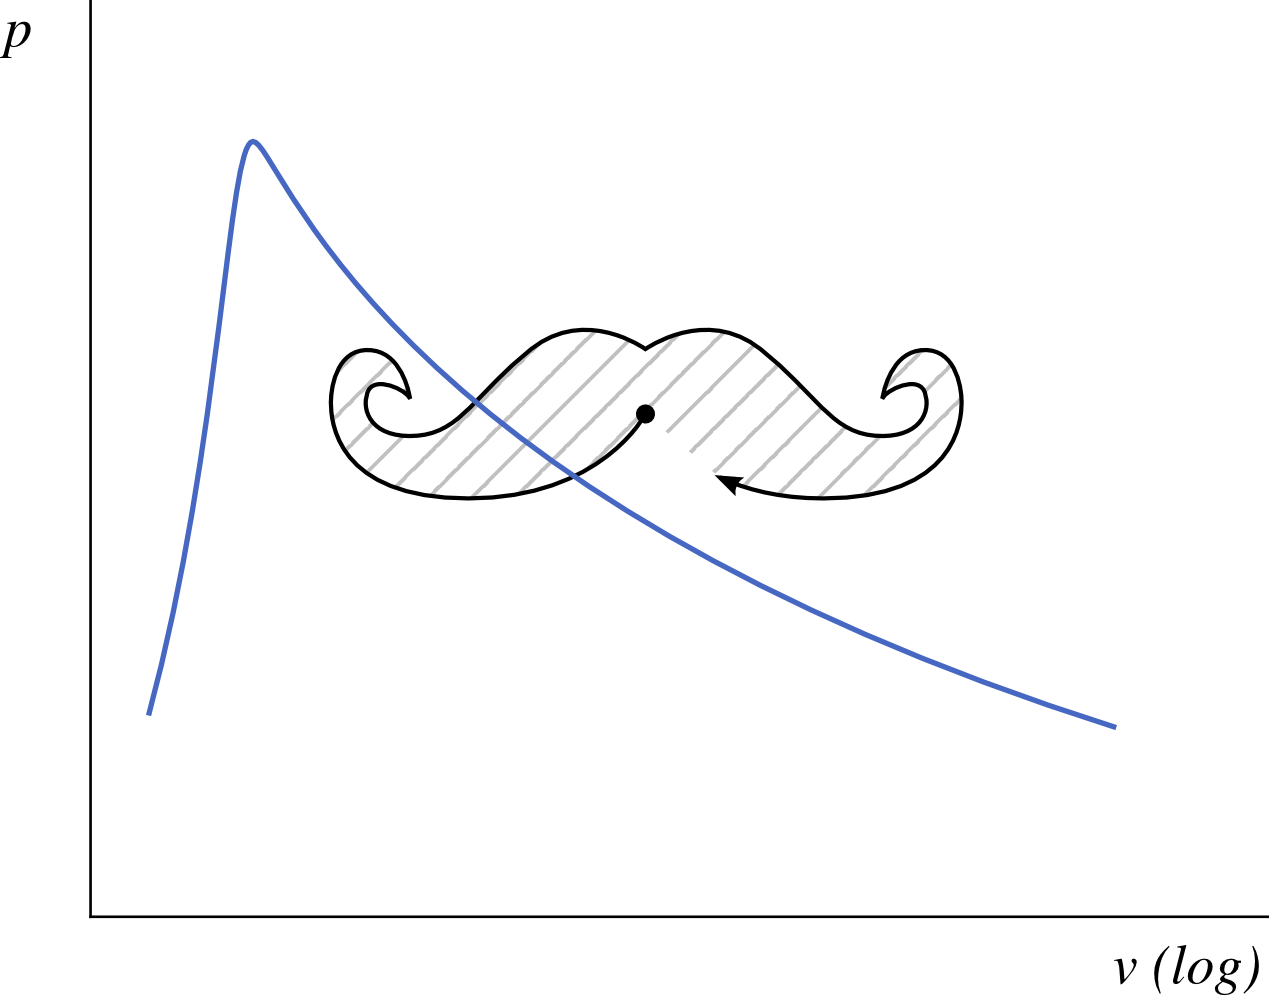
\includegraphics[width=\pvdiagramwidth]{images/pv_lv_moustache.png}
			\end{center}
			\supercaption{Évolution entièrement arbitraire d’un liquide/vapeur représentée sur un diagramme pression-volume. Outre un sens de l’humour déplorable, une telle évolution requiert une combinaison extrêmement complexe de transferts de chaleur et de travail que l’étudiant/e est invité/e à se représenter.}{\cczero \oc}
			\label{fig_lv_pv_moustache}
		\end{figure}
		
		Nous nous sommes concentrés sur quatre évolutions particulières, parce qu’elles jouent chacune un rôle important, pour les physiciens et pour les ingénieurs, dans la conception des machines thermiques. En contrôlant astucieusement les transferts de chaleur et de travail, on peut bien sûr provoquer n’importe quelle évolution arbitraire.

